\documentclass[%
reprint,
superscriptaddress,
%groupedaddress,
%unsortedaddress,
%runinaddress,
%frontmatterverbose, 
%preprint,
%preprintnumbers,
%nofootinbib,
%nobibnotes,
%bibnotes,
 amsmath,amssymb,
 aps,
 prx,
%pra,
%prb,
%rmp,
%prstab,
%prstper,
longbibliography,
floatfix,
]{revtex4-2}
\usepackage{amsmath}
\usepackage{braket}
\usepackage{geometry}
\usepackage{amssymb}
\usepackage{amsfonts}
\usepackage{mathtools}
\usepackage{appendix}
\usepackage{url}
%\usepackage{floatrow}
\usepackage[utf8]{inputenc}
\usepackage{array}

\usepackage[dvipsnames]{xcolor}\usepackage[draft]{changes} %%%%---annotations are visible
\usepackage{color}   %May be necessary if you want to color links
\usepackage{hyperref}
\hypersetup{
    colorlinks=true, %set true if you want colored links
    linktoc=all,     %set to all if you want both sections and subsections linked
    linkcolor=blue,  %choose some color if you want links to stand out
}

\geometry{
 a4paper,
 total={170mm,257mm},
 left=20mm,
 top=20mm,
 }
 \usepackage{graphicx} 
%\usepackage{authblk}

\newcommand{\ER}[1]{{\color{blue}{{}[ER: #1]}}}
\newcommand{\sh}[1]{{\color{blue}{{}[SS: #1]}}}%for comments
\newcommand{\singh}[1]{{\color{orange}{{}#1}}}%for recommended edits
\newcommand{\gil}[1]{{\color{blue}{{}[GR: #1]}}}
\newcommand{\AC}[1]{{\color{blue}{{}[AC: #1]}}}


\usepackage{orcidlink}

\begin{document}
\preprint{APS/123-QED}
\title{Impact of Josephson Junction Array modes on Fluxonium Readout}

\author{Shraddha Singh\orcidlink{0000-0002-4921-1410}}\thanks{Corresponding email: shraddha.singh@yale.edu}
\affiliation{Department of Applied Physics and Physics, Yale University, New Haven, Connecticut 06511, USA}
\affiliation{Yale Quantum Institute, Yale University, New Haven, Connecticut 06511, USA}
\affiliation{AWS Center for Quantum Computing, Pasadena, CA 91125, USA}
\author{Gil Refael}
\affiliation{AWS Center for Quantum Computing, Pasadena, CA 91125, USA}
\affiliation{Institute for Quantum Information and Matter,
California Institute of Technology, Pasadena, CA 91125}
\author{Aashish Clerk}
\affiliation{Pritzker School of Molecular Engineering, University of Chicago, Chicago, Illinois 60637, USA}
\affiliation{AWS Center for Quantum Computing, Pasadena, CA 91125, USA}
\author{Emma Rosenfeld}\thanks{Present address: Google Research}
\affiliation{AWS Center for Quantum Computing, Pasadena, CA 91125, USA}
\date{\today}%remove this eventually

\begin{abstract}
Dispersive readout of superconducting qubits is often limited by non-ideal backaction effects in which the readout drive induces unwanted transitions between qubit levels.  While there is a growing understanding of such effects in transmon qubits, the case of highly nonlinear fluxonium qubits is more complex.  We theoretically analyze measurement-induced state transitions (MIST) during the dispersive readout of a fluxonium qubit, focusing on a new mechanism: the possibility of transitions where the drive simultaneously excites an internal mode of the Josephson junction array in the fluxonium circuit, while also causing a qubit transition. Using an adiabatic Floquet approach, we show that these new kinds of MIST processes, which we refer to as p-MIST, are relevant at particular values of realistic circuit parameters and relatively low readout drive powers.  As we show, they can also contribute to excess qubit dephasing even after a measurement is complete. In a study of mitigation strategies, we highlight readout frequency choices which avoid p-MIST, and analyze the dependency of qubit-parasitic mode coupling on different circuit parameters. Our results underscore the impact of parasitic modes on qubit performance in highly anharmonic superconducting circuits, especially if they are not carefully treated during circuit design while choosing the readout drive frequency.
\end{abstract}

\maketitle
\section{Introduction}
%%%General fluxonium background%%%%

The fluxonium superconducting qubit, based on a Josephson junction shunted by a capacitor and a large inductance, has emerged as an extremely promising platform for quantum information. It exhibits extremely long lifetimes~\cite{high_coherence_2019, somoroff_millisecond_2023, single_cooper_pair, earnest_realization_2018}, and both single~\cite{zhang_universal_2021} and two-qubit gates~\cite{ding_high-fidelity_2023, zhang_tunable_2024} have been demonstrated with high fidelity, with potential room for even further improvements~\cite{nesterov_cnot_2022, nesterov_proposal_2021, dogan_two-Fluxonium_2023, rosenfeld_designing_2024, nguyen_blueprint_2022}. The inductive shunt is a crucial part of the fluxonium circuit, with the most common realization being a Josephson junction array (JJA); in regimes where internal array modes are not excited, the JJA can act as a linear superinductance (see e.g.~\cite{masluk_microwave_2012, wang_achieving_2024}).       

In addition to coherence and the ability to do high-fidelity gates, the ability to make fast and efficient measurements is crucial to any qubit platform.  Similar to other superconducting qubits, dispersive readout (using a driven readout resonator) has been the standard choice for fluxonium readout 
(see e.g.~\cite{{zhang_universal_2021}}).  While such measurement schemes should ideally be quantum non-demolition (QND)~\cite{blais2021circuit}, some experiments have reported non-QND backaction (either enhanced relaxation or transitions to non-computational states) during fluxonium readout~\cite{ding_high-fidelity_2023, gusenkova2021quantum,vooldriving2018,voolnon2014}.  This is similar to the situation with dispersive readout with more standard transmon qubits, where similar effects have long been seen.  Recent theoretical work on driven transmon qubits has provided strong insights into these so-called measurement-induced state transitions (MIST), showing that multi-photon transitions can lead to resonant excitation of the transmon to higher levels (see e.g.~\cite{shillito2022dynamics,xiao2023diagrammatic,khezri2023measurement,cohen2023reminiscence,dumas2024unified,sank2016measurement}).

%%%%%%%%%%%%%%%%%%%%%%%%%%%%%%%%%%%%%
\begin{figure}
    \centering
    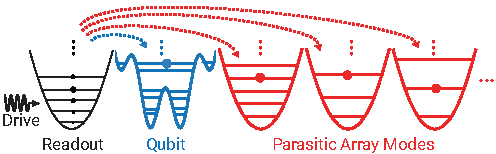
\includegraphics[width=\linewidth]{Figures/Demo.pdf}
    \caption{A parasitic effect where energy in a coherent state of the driven readout mode (black) excites extraneous linear modes (red) and the nonlinear qubit mode (blue) simultaneously. 
    }
    \label{fig:demo}
\end{figure}
%%%%%%%%%%%%%%%%%%%%%%%%%%%%%%%%%%%%%


Given that similar MIST-like effects have been seen in fluxonium qubits, it is only natural to want a similar theoretical understanding of the relevant mechanisms, to ultimately find means for suppressing such effects.  There are of course significant differences between fluxonium and the transmon, which will significantly alter MIST physics.  For example, the enhanced nonlinearity can dramatically change the number and likelihood of potential transitions \cite{nesterov2024measurement,xiao2023diagrammatic}.  In this work, we provide a comprehensive analysis of another new MIST mechanism in fluxonium:  additional MIST transitions of the qubit that arise due to the internal modes of the JJA in the fluxonium circuit (see Fig.~\ref{fig:demo}). We show that for realistic parameters and drive powers, deleterious resonant processes that simultaneously excite the qubit and an internal mode can indeed occur; we term these processes parasitic-mode induced state transitions (p-MIST).  One can view this as an example of an even more general problem: how is MIST physics modified in the presence of a structured environment?  

We focus on a heavy fluxonium qubit operated at its flux sweet spot (c.f.~Fig.~\ref{fig:meas_circuit}) and study MIST effects keeping the coupling to the most relevant JJA internal modes.  Similar to studies of MIST in transmons~\cite{cohen2023reminiscence,dumas2024unified}, we treat the readout as an effective classical drive on the fluxonium-plus-JJA system and use an adiabatic Floquet branch analysis to identify dominant MIST processes. We also validate this approach through full-time-dependent simulations.  
Our work goes beyond simply showing that such processes could be relevant. We discuss how they could provide a mechanism for degrading qubit coherence even after measurements are complete (via dephasing from dispersive couplings to the excited internal modes).  We also discuss how alternate circuit designs could be employed to help minimize p-MIST processes, paying special attention to how modifications affect the parasitic mode to qubit coupling strengths.  Our analysis here suggests that once one considers readout, parasitic JJA modes introduce additional constraints on the circuit design for highly coherent fluxonium qubits.     

%%%%%structure%%%%%%
The remainder of this article is structured as follows. Sec.~\ref{sec:Fluxonium}
provides an analysis of the full circuit including fluxonium, JJA, and readout resonator.  Using a standard harmonic approximation, we derive qubit-parasitic mode coupling strengths, and lower bound parasitic mode effects during readout. Sec.~\ref{sec:MIST} analyzes readout dynamics, including MIST processes and dephasing from parasitic modes. Sec.~\ref{sec:expressions} analyzes the effects of varying coupling strengths on p-MIST, and investigates different ranges of readout frequencies and parasitic mode frequencies using an energy-conservation picture. Finally, in the concluding Sec.~\ref{sec:conclusion} we discuss directions for future work that build upon our analysis.

%%%%%%%%%%%%%%%%%%%%%%%%%%%%%%%%%
\begin{figure}[t]
\centering    
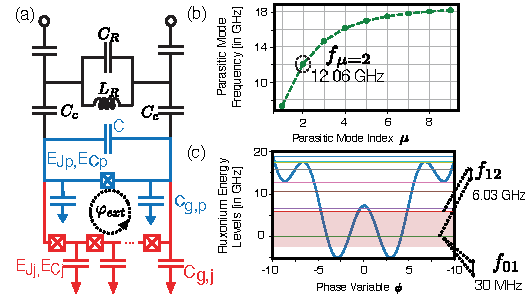
\includegraphics[width=\linewidth]{Figures/Meas_Circuit.pdf}
\caption{(a) Fluxonium readout circuit. The color scheme shows primary components that correspond to various modes, shown in Fig.~\ref{fig:demo} when a JJA fluxonium circuit is connected to a readout resonator (R). The subscripts $p,j$ denote components of the phase-slip junction and the JJA, respectively. This circuit shows coupling capacitances ($C_c$), readout frequency parameters ($\omega_r=1/\sqrt{L_{R}C_{R}}$), parasitic ground capacitances in JJA ($C_{g,j}$) and next to the phase-slip junction ($C_{g,p}$). The differential capacitance $C$ adjusts the charging energy of the qubit mode (see Table~\ref{tab:readout_params}). (b) Fluxonium mode energy levels in units of $h$, with the highlighted area showing the first three levels essential for certain readout schemes~\cite{zhang_universal_2021}. (c) Parasitic mode frequencies $\omega_\mu/2\pi$. The lowest even mode $\mu = 2$ has the strongest coupling to the qubit (see Fig.~\ref{fig:coupling-strength}). 
}
\label{fig:meas_circuit}
\end{figure}
%%%%%%%%%%%%%%%%%%%%%%%%%%%%%%%%%

%%%%%%%%%%%%%%%%%%%%%%%%%%%%%%%%%
\renewcommand{\arraystretch}{1.5} % Adjust the value as needed
\begin{table}[htb]
\centering
\begin{tabular}{|c|c|c|c|c|c|c|c|c|c|}
    \hline
     $N$ & $\varphi_{ext}$ & $E_{J_p}$ & $E_{C_p}$ & $E_C$ & $E_{C_j}$ & $E_{J_j}$ & $E_{C_{g,j}}$ & $E_{C_{g,p}}$ & $E_c$ \\
    \hline
    $122$ & $0.5\Phi_0$ & $7.30$ & $1.46$ & $17$ & $0.74$ & $60$ & $194$ & $1.94$ & $19.40$ \\
    \hline
\end{tabular}
\caption{Circuit parameters for Fig.~\ref{fig:meas_circuit}(a) inspired by Ref.~\cite{zhang_universal_2021}. All energies are given in GHz. Here $\Phi_0=h/2e$ denotes the magnetic flux quantum. The capacitive energies $E_{C'}=\frac{19.4}{{C'}(\mathrm{fF})} \ \mathrm{GHz}$ are computed from the corresponding capacitances $C'$. See Table~\ref{tab:params} in App.~\ref{app:Hamiltonian} for the values of capacitances.}
\label{tab:circuit_params}
\end{table}
%%%%%%%%%%%%%%%%%%%%%%%%%%%%%%%%%



%%%%%%%%Our techniques and observations%%%%%%%%%%%%%




\renewcommand{\arraystretch}{1.5} % Adjust the value as needed

%%%%%%%%%%%%%%%%%%
\begin{table*}[tb]
    \centering
\begin{tabular}{|c|c|c|c|c|c|c|c|c|c|c|c|c|}
    \hline
    \textbf{Qubit ($\phi$) $\&$}&$\omega_{01}/2\pi$&$\omega_{12}/2\pi$ &$\tilde{E}^\phi_c$ &$g_{\phi r}/2\pi$&$\chi_{\phi r}(01)/2\pi$&$\chi_{\phi r}(12)/2\pi$&$\omega_r/2\pi$&$\kappa_r/2\pi$\\
    \cline{2-9}
\textbf{Readout ($r$)}&$30 \ \mathrm{MHz}$& $6.04 \ \mathrm{GHz}$ & $0.92 \ \mathrm{GHz}$& $25.50 \ \mathrm{MHz}$& $0.18 \ \mathrm{MHz}$&$0.98 \ \mathrm{MHz}$&$8.50 \ \mathrm{GHz}$&$1 \ \mathrm{MHz}$\\    
\hline\textbf{Parasitic-Mode} & \multicolumn{2}{c|}{} & $g_{\phi\mu}/2\pi$&$g_{\mu r}/2\pi$&$\chi_{\phi\mu}(01)/2\pi$&$\chi_{\phi\mu}(12)/2\pi$&$\omega_\mu/2\pi$&$Q_\mu$\\
    \cline{4-9}
\textbf{($\mu=2$)}&\multicolumn{2}{c|}{} &$157 \ \mathrm{MHz}$& $4.22 \ \mathrm{MHz}$& $-1.10 \ \mathrm{MHz}$& $5 \ \mathrm{MHz}$& $12.06 \ \mathrm{GHz}$&$10^{4}$\\    
\hline
\end{tabular}
\caption{Measurement parameters for qubit mode $\phi$, readout mode $r$ and closest even parasitic mode $\mu=2$.  All quantities are derived and computed analytically using circuit parameters listed in Table~\ref{tab:circuit_params} (see Apps.~\ref{app:alt_circuits}-\ref{app:Hamiltonian} for details). \textbf{Qubit-Readout Parameters:} ($\omega_{ij}$) qubit $i\rightarrow j$ splitting frequency between fluxonium excited states $i, j$; ($\tilde{E}^\phi_c$) qubit charging energy; ($g_{\phi r}$) qubit-readout coupling; ($\chi_{\phi r}(ij)$) dispersive shift due to readout mode in the two-level $ij$ system; ($\omega_r$) readout mode frequency; ($\kappa_r$) decay rate of the readout resonator. \textbf{Parasitic-Mode Parameters:} ($g_{\phi \mu}$) qubit-parasitic coupling; ($g_{\mu r}$) parasitic-readout coupling; ($\chi_{\phi \mu}(ij)$) dispersive shift due to parasitic mode $\mu$ in the two-level $ij$ system; ($\omega_\mu$) mode frequency; and ($Q_\mu$) internal quality factor inspired by~\cite{masluk_microwave_2012}.}   \label{tab:readout_params}
\end{table*}
%%%%%%%%%%%%%%%%%%



%%%%%%%%%%%%%%%%%%%%%%%%%%%%%%%%%%%%%%%%%%%%%%%%%%%%%%%%%%%%%%%%%
%%%%%%%%%%%%%%%%%%%%%%%%%%%%%%%%%%%%%%%%%%%%%%%%%%%%%%%%%%%%%%%%%
%%%%%%%%%%%%%%%%%%%%%%%%%%%%%%%%%%%%%%%%%%%%%%%%%%%%%%%%%%%%%%%%%

\section{Fluxonium Readout Circuit}\label{sec:Fluxonium}


%%%%Fluxonium circuit%%%%%%%%%%%%%%%%%%%%%%
We consider a JJA-fluxonium circuit dispersively coupled to a readout mode as shown in Fig.~\ref{fig:meas_circuit}. We chose circuit parameters (as listed in Table~\ref{tab:circuit_params}) motivated by recent experiments on heavy fluxonium~\cite{zhang_tunable_2024,zhang_universal_2021, ding_high-fidelity_2023}.  We also restrict attention to the flux ``sweet spot" that maximizes qubit coherence.
This choice is also expected to reduce the number of allowed transitions in the circuit, as transitions between parity-conserving states via first-order processes are forbidden in this case. For our parameters, the qubit frequency ($\omega_{01}/2\pi$) is $\sim 30 \ \mathrm{MHz}$ and the plasmon frequency (i.e.~splitting frequency between first and second qubit excited states $\omega_{12}/2\pi$) is $\sim 6 \ \mathrm{GHz}$ (see Table~\ref{tab:readout_params} for a full list of readout parameters).
 

%%%%%%%%%JJA+assumptions%%%%%%%%%%%%%%%%
Our work specifically investigates the role of the JJA, which comprises the inductive shunt of the fluxonium. The array comprises $N$ junctions and $N-1$ ground capacitances($C_{g_i}$)~\cite{manucharyan2009fluxonium}. We neglect disorder effects, and take junction parameters and parasitic ground capacitances to be uniform in the array (i.e.~$C_{g_1}=..=C_{g_{N}}$). This capacitance value is given by $C_{g,j}$ where the subscript $j$ indicates the parasitic ground capacitance in the JJA~\footnote{Note that the ground capacitances $C_{g_n}$ are distinct from the self-capacitance $\frac{19.4}{E_{C,j}(\mathrm{GHz})}\mathrm{fF}$ (see Table~\ref{tab:params}) across the junctions in the array, which set the junction array plasmon frequency \cite{catelani2011relaxation}}. As shown in Fig.~\ref{fig:meas_circuit}(a), 
two additional identical ground capacitances $C_{g_0}, C_{g_N}$ near the phase-slip junctions may have different values compared to those in the interior of the array, i.e.~
$C_{g_0}=C_{g_N}\equiv C_{g,p}\neq C_{g, j}$. Note that the subscript $p$ indicates the parasitic ground capacitances next to the phase-slip junction.

The JJA fluxonium circuit has $N$ internal degrees of freedom~\cite{ferguson2013symmetries,viola2015collective}: one qubit mode ($\phi$) and $N-1$ internal modes ($\mu=1,2,...,N-1$). These  internal modes are coupled via the ground capacitances and are referred to as the ``parasitic" modes of the JJA. 
% notation
In our notation, we label the readout mode as $r$. The charge and flux quadratures of the qubit mode are denoted by $\hat N_\phi$ and $\hat \phi$ where $[\hat \phi,\hat N_\phi]=i\hbar$. We simplify the problem by treating all but the qubit mode as harmonic oscillators as assumed in previous works~\cite{ferguson2013symmetries,viola2015collective,dumas2024unified}. We expect that this assumption will lower bound the effects of JJA parasitic modes on qubit performance for driven fluxonium circuits. We denote the photon loss and gain operators of the linear modes $r,\mu$ using $\hat a_r,\hat a_\mu$ and $\hat a_r^\dagger,\hat a_\mu^\dagger$, respectively. 

Setting $\hbar=1$, the Hamiltonian of our fluxonium circuit has the form~\cite{viola2015collective} (see App.~\ref{app:alt_circuits} for derivation)

\begin{equation}
   \hat H =\hat{H}_\phi + \hat{H}_\mu + \hat{H}_r + \hat{H}_{int},\label{Hamiltonian_total}
\end{equation}
where the qubit Hamiltonian $\hat{H}_\phi$ (with JJA inductive energy $E_L=E_{J_j}/N$) is 
\begin{equation}
\hat{H}_\phi / 2\pi = 4\tilde{E}^\phi_c \hat N_\phi^2+ E_{J_p}\cos{\hat\phi}+E_L\hat \phi^2 /2,\label{eq:Hphi}
\end{equation}
the junction array and readout Hamiltonians are $\hat{H}_\mu = \sum_{\mu}\omega_\mu \hat a_\mu^\dagger \hat a_\mu$ and $\hat{H}_r = \omega_r \hat a_r^\dagger \hat a_r$, respectively. The qubit charging energy
$\tilde{E}^\phi_c$ (see Table~\ref{tab:readout_params}) deviates from the target value of $E_c^{\phi}=1 \ \mathrm{GHz}$ due to parasitic capacitance. The coupling between the three modes is described by the interaction Hamiltonian
\begin{align}\label{eq:int_hamiltonian}
\hat{H}_{int} &= \sum_{\mu} g_{\phi\mu} \frac{\hat N_\phi}{{N_{\phi,\mathrm{ZPF}}}} (\hat a_\mu-\hat a_\mu^\dagger)\nonumber \\ &\quad-g_{\phi r} \frac{\hat N_\phi}{{N_{\phi,\mathrm{ZPF}}}} (\hat a_r-\hat a_r^\dagger) \nonumber \\&\quad- \sum_{\mu} g_{\mu r} (\hat a_r-\hat a_r^\dagger)(\hat a_\mu-\hat a_\mu^\dagger).
\end{align}
where for our parameters, the zero-point fluctuations of qubit charge  $N_{\phi,\mathrm{ZPF}}=0.36$. Values for all remaining parameters appearing here are given in Table~\ref{tab:readout_params}. Explicit expression for $g_{\phi\mu}$ is discussed in Sec.~\ref{sec:expressions}, while expressions for all other variables can be found in App.~\ref{app:Hamiltonian}.

In this Hamiltonian derivation, we have used the conclusion from Ref.~\cite{viola2015collective} that the symmetry of the parallel circuit in Fig.~\ref{fig:meas_circuit}(a) prevents coupling between odd parasitic modes (including $\mu=1$) and other circuit modes. We extend this result to two additional circuits, with different ground circuit configurations, showing qualitatively consistent conclusions across all three circuits in App.~\ref{app:alt_circuits}. The circuits yield the same Hamiltonian when the differential capacitance $C$ and coupling capacitance $C_c$ are altered such that qubit frequency and qubit-readout coupling are the same across all three circuits (see Table~\ref{tab:parasitic_params} in App.~\ref{app:alt_circuits}). 
 
%%%%%choosing the lowest even mode %%%%%
 We find that the lowest-frequency even parasitic mode $\mu=2$ has the strongest coupling to the qubit mode (see Fig.~\ref{fig:coupling-strength} in App.~\ref{app:coupling}); parameters for which are listed in Table~\ref{tab:readout_params}. Moreover, Fig.~\ref{fig:coupling-strength} shows that the $\mu=2,4,6$ parasitic modes couple to the qubit with a strength $g_{\phi\mu}$ that is stronger than the qubit-readout coupling $g_{\phi r}$. This relative behavior between coupling strengths has also been pointed out previously in Ref.~\cite{viola2015collective}.
 
 Given the above insights and our stated goal of understanding readout-induced transitions that involve the parasitic modes, in the rest of this work we will focus on the parallel circuit from Fig.~\ref{fig:meas_circuit} using parameters given by Tables~\ref{tab:circuit_params}-\ref{tab:readout_params} in Eq.~\ref{Hamiltonian_total}.  Further, our description will only retain the strongest coupled parasitic mode $\mu = 2$, along with the qubit and readout resonator.  For details on other parasitic modes and their parameters, see App.~\ref{app:coupling}. Note that for our chosen parameters (see Table~\ref{tab:circuit_params}), the qubit couples roughly six times more strongly to the parasitic mode at $\mu=2$ than it does to the readout $r$~\footnote{In fact, the first four even parasitic modes with coupling strengths within a factor of $10$ of $g_{\phi r}$. See Fig.~\ref{fig:coupling-strength} in App.~\ref{app:coupling}}.  As we will show, this strong coupling implies that the parasitic mode can play a strong role in measurement-induced state transitions, i.e. the p-MIST effect that is the subject of this work.   

\section{Parasitic-mode-Induced State Transitions: p-MIST}\label{sec:MIST}

In this section, we analyze how the presence of a parasitic mode ($\mu=2$) affects the dynamics of a driven fluxonium circuit during a readout pulse. To simulate the linear drive on the readout resonator, we add a drive term $\hat{V}_d=i\xi (\hat a_r-\hat a_r^\dagger)\cos{\omega_d t}$ to the system Hamiltonian in Eq.~\ref{Hamiltonian_total}. If we consider the fluxonium qubit mode, parasitic modes, and readout resonator, a full numerical analysis of several excitations in the circuit would require a prohibitively large Hilbert space. To truncate our Hilbert space to feasible dimensions for numerical simulations, here we only include a single parasitic mode $\mu=2$ (as previously justified in Sec.~\ref{sec:Fluxonium}), and we replace the readout mode with a classical drive term~\cite{cohen2023reminiscence,dumas2024unified,xiao2023diagrammatic} (see derivation in App.~\ref{app:semi-classical}). Under this semi-classical approximation, the driven circuit Hamiltonian includes the qubit mode $\phi$ and the parasitic mode at $\mu=2$, and is
\begin{align}
  \hat H_{s.c.}(\bar n_r)=\hat H_0+\hat V_{s.c.}(\bar n_r).  \label{eq:drive_Ham}
\end{align}
Here, the bare Hamiltonian is
\begin{align}
H_0=\hat H_\phi+\hat H_{\mu}-\frac{g_{\phi\mu}}{N_{\phi,\mathrm{ZPF}}} \hat N_\phi (\hat a_{\mu}-\hat a_{\mu}^\dagger) \label{eq:bare_ham} 
\end{align}
and the modified drive term $V_{s.c.}$ is
\begin{align}
    \hat V_\textrm{s.c.}(\bar n_r)&=\frac{\xi_{\phi r}(\bar n_r)}{N_{\phi,\mathrm{ZPF}}} \hat N_\phi\cos{\omega_d t}+\frac{\xi_{\mu r}(\bar n_r)}{N_{\mu, \mathrm{ZPF}}} \hat N_\mu\cos{\omega_d t}\label{eq:drive},
\end{align}
where $\xi_{\mu(\phi) r}(\bar n_r)=2g_{\mu(\phi) r}\sqrt{\bar n_r}$, and $\bar n_r$ denotes the average number of photons in the readout cavity. In the remaining text, we refer to the quantities $\xi_{\phi r/\mu r}$ as  ``qubit drive strengths" and ``parasitic drive strengths", respectively. And, the squared quantities $|\xi_{\mu(\phi) r}|^2$ will be termed as effective drive powers.

Our primary focus is to analyze p-MIST processes that introduce simultaneous transitions in the parasitic mode and the qubit mode. To identify the likely state transitions in the driven circuit, we first examine the energy eigenstates of the bare Hamiltonian $\hat{H}_0$ in Eq.~\ref{eq:bare_ham}. These states will be hybridized fluxonium-parasitic mode states, and we label them as $\ket{\tilde{k}, \tilde{n}}$.  A given state $\ket{\tilde{k}, \tilde{n}}$ corresponds to the eigenstate that has the maximum overlap with ``bare" fluxonium and parasitic mode states $\ket{k}_\phi\otimes\ket{n}_\mu$, i.e., the eigenstates of $H_{\phi}$ and $H_{\mu}$.

In what follows, we identify relevant state transitions in the driven fluxonium plus parasitic mode system. First, we perform an analysis based on the Floquet eigenstates of our system at a given fixed drive power.  Similar to Refs.~\cite{khezri2023measurement,cohen2023reminiscence,dumas2024unified} for transmons, we can use this to then simulate the drive ring-up to some chosen final photon number $\bar{n}_r$, and identify potential state transitions.  We do this for a range of drive frequencies $\omega_d$. We find that the presence of the parasitic mode $\mu=2$ significantly increases the number of MIST processes in the system. We analyze the processes that cause these transitions and quantify their rates using perturbative approaches and Landau Zener probability calculations~\cite{ikeda2022floquet}. We also show that the residual population in the parasitic modes, after a readout pulse, can lead to significant dephasing of the reset qubit mode, limiting the performance of the qubit for future use.

%%%%%%%%%%%%%%%%%%%%%%%%%%%%%%%%%%
\subsection{Recap of the Floquet branch analysis method} 

%%%%%%%%%%%%%%%%%%%%%%%%%%%%%%%%%%
\begin{figure}[!htb]
    \centering
    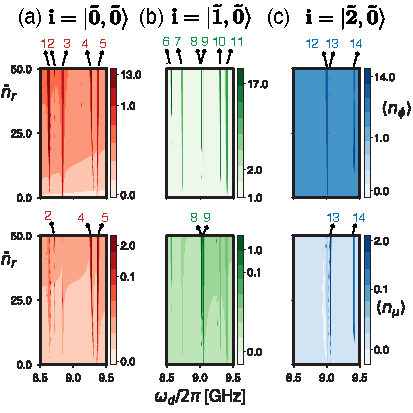
\includegraphics[width=0.5\textwidth]{Figures/Floquet_min.pdf}
    \caption{{\bf MIST and p-MIST processes as seen in Floquet branch simulations.}  
    Each column corresponds to the branch associated with a specific undriven (but dressed) eigenstate $i=\ket{\tilde{k},\tilde{0}}$.  
    \textbf{Top row:} Average fluxonium excitation number in the given branch $\langle n_\phi\rangle $, as a function of drive power ($\propto\bar{n}_r$) and drive frequency $\omega_d$. \textbf{Bottom row:} Average excitation number of the $\mu=2$ parasitic mode, $\langle n_\mu\rangle$. Color scales use a log scaling to help visualize all transitions.  Arrows and numbers are used to indicate each transition (with numbers corresponding to Table~\ref{tab:p-MIST}). See Figs.~\ref{fig:Trans0}-\ref{fig:Trans2} of App.~\ref{app:Floquet-trans} for corresponding behaviour of  quasienergies.}
    \label{fig:Floquet}
\end{figure}
\begin{table*}[t]
    \centering
    \begin{tabular}{w{c}{2.0cm}w{c}{3.0cm}w{c}{2.0cm}w{c}{2.0cm}w{c}{2.5cm}w{c}{1.5cm}w{c}{2.5cm}}
\hline
\shortstack{\\\textbf{Transition }\\\textbf{No.}\\\textbf{ (see Fig.~\ref{fig:Floquet})}} &\shortstack{\\\textbf{Fluxonium}\\\textbf{MIST}\\\textbf{Process}} &\shortstack{\\\textbf{Threshold}\\\textbf{Drive}\\\textbf{Photon ($\bar n_r$)}}& \shortstack{\\\textbf{Drive}\\\textbf{Frequency}\\($\omega_d/2\pi$)}& \shortstack{\\\textbf{Quasienergy}\\\textbf{Gap}\\($\Delta_{ac}$)}& \textbf{p-MIST}&\shortstack{\textbf{Drive Photons}\\\textbf{Absorbed}\\\textbf{(see Fig.~\ref{fig:trans_prof})}}\\
\hline
\rule{0pt}{4ex}$1.$&$\color{BrickRed}{\ket{\tilde{0},\tilde{0}}}$$\xleftrightarrow []{\hspace{1em}}\ket{\tilde{13},\tilde{0}}$&$13$ &$8.64 \ \mathrm{GHz}$&$0.90 \ \mathrm{MHz}$&$\times$ & $3$\\
%\hline
$2.$&$\color{BrickRed}{\ket{\tilde{0},\tilde{0}}}$$\xleftrightarrow[]{\hspace{1em}}\ket{\tilde{4},\tilde{2}}^*$ &$48$&$8.71 \ \mathrm{GHz}$&$0.06 \ \mathrm{MHz}$&$\color{BrickRed}{\checkmark}$ & $4$\\
%\hline
$3.$&$\color{BrickRed}{\ket{\tilde{0},\tilde{0}}}$$\xleftrightarrow[]{\hspace{1em}}\ket{\tilde{8},\tilde{0}}$ &$\sim 0$&$8.84 \ \mathrm{GHz}$&$-$&$\times$ &$2$\\
%\hline
$4.$&$\color{BrickRed}{\ket{\tilde{0},\tilde{0}}}$$\xleftrightarrow[]{\hspace{1em}}\ket{\tilde{6},\tilde{1}}^*$&$46$&$9.25 \ \mathrm{GHz}$&$1.63 \ \mathrm{MHz}$&$\color{BrickRed}{\checkmark}$ &$2$\\
$5.$&$\color{BrickRed}{\ket{\tilde{0},\tilde{0}}}$$\xleftrightarrow[]{\hspace{1em}}\ket{\tilde{3},\tilde{1}}$ &$12$&$9.36 \ \mathrm{GHz}$&$0.56 \ \mathrm{MHz}$&$\color{BrickRed}{\checkmark}$ &$2$\\
%\hline
$6.$&$\color{ForestGreen}{\ket{\tilde{1},\tilde{0}}}$$\xleftrightarrow[]{\hspace{1em}}\ket{\tilde{17},\tilde{0}}$ &$32$&$8.56 \ \mathrm{GHz}$&$0.25 \ \mathrm{MHz}$&$\times$ & $4$\\
%\hline
$7.$&$\color{ForestGreen}{\ket{\tilde{1},\tilde{0}}}$$\xleftrightarrow[]{\hspace{1em}}\ket{\tilde{7},\tilde{0}}$ &$4$&$8.73 \ \mathrm{GHz}$&$0.74 \ \mathrm{MHz}$&$\times$ & $2$\\
%\hline
$8.$&$\color{ForestGreen}{\ket{\tilde{1},\tilde{0}}}$$\xleftrightarrow[]{\hspace{1em}}\ket{\tilde{12},\tilde{1}}$&$19$&$9.02 \ \mathrm{GHz}$&$0.12 \ \mathrm{MHz}$&$\color{ForestGreen}{\checkmark}$ & $4$\\
%\hline
$9.$&$\color{ForestGreen}{\ket{\tilde{1},\tilde{0}}}$$\xleftrightarrow[]{\hspace{1em}}\ket{\tilde{2},\tilde{1}}$  &$11$&$9.05 \ \mathrm{GHz}$&$0.66 \ \mathrm{MHz}$&$\color{ForestGreen}{\checkmark}$ & $2$\\
%\hline
$10.$&$\color{ForestGreen}{\ket{\tilde{1},\tilde{0}}}$$\xleftrightarrow[]{\hspace{1em}}\ket{\tilde{14},\tilde{0}}$ &$7$&$9.31 \ \mathrm{GHz}$&$0.50 \ \mathrm{MHz}$&$\times$ & $3$\\
%\hline
$11.$&$\color{ForestGreen}{\ket{\tilde{1},\tilde{0}}}$$\xleftrightarrow[]{\hspace{1em}}\ket{\tilde{9},\tilde{0}}$ &$2$&$9.41 \ \mathrm{GHz}$&$1.19 \ \mathrm{MHz}$&$\times$ &$2$\\
%\hline
$12.$&$\color{RoyalBlue}{\ket{\tilde{2},\tilde{0}}}$$\xleftrightarrow[]{\hspace{1em}} \ket{\tilde{12},\tilde{0}}$ &$3$&$9.00 \ \mathrm{GHz}$&$0.73 \ \mathrm{MHz}$&$\times$ & $2$\\
%\hline
$13.$&$\color{RoyalBlue}{\ket{\tilde{2},\tilde{0}}}$$\xleftrightarrow[]{\hspace{1em}}\ket{\tilde{0},\tilde{2}}$&$38$&$9.06 \ \mathrm{GHz}$&$0.53 \ \mathrm{MHz}$&$\color{RoyalBlue}{\checkmark}$ & $2$\\
%\hline
$14.$&$\color{RoyalBlue}{\ket{\tilde{2},\tilde{0}}}$$\xleftrightarrow[]{\hspace{1em}}\ket{\tilde{5},\tilde{1}}^*$ &$49$&$9.41 \ \mathrm{GHz}$&$2.71 \ \mathrm{MHz}$&$\color{RoyalBlue}{\checkmark}$ & $2$\\
\hline
\end{tabular}
\caption{Measurement-induced-state-transition (MIST) observed in Fig.~\ref{fig:Floquet}. Column $1$ lists the numbering used to mark the transitions in Fig.~\ref{fig:Floquet}. Here $\ket{\tilde{i},\tilde{j}}$ indicates the hybridized eigenstate of $H_0$ (see Eq.~\ref{eq:bare_ham}) which has the maximum overlap with the state $\ket{i}_\phi\otimes \ket{j}_{\mu=2}$ in the disjoint Hilbert space of qubit mode ($\phi$) and parasitic mode ($\mu=2$). Column $2$ lists the MIST processes that start  at the lowest average readout photon number $\bar n_r$ given by column $3$. In some cases, we use $\bar n_r\sim 0$ to indicate that the drive frequency is exactly resonant with the transition frequency \singh{between the two levels}. A `$^*$'-marked state indicates hybridization at lower $\bar n_r$ due to preceding transitions~\footnote{$\ket{\tilde{4},\tilde{2}}^*:\ket{\tilde{4},\tilde{2}}\xleftrightarrow[]{\hspace{1em}}\ket{\tilde{14},\tilde{2}}$ at $\bar n_r=5, \omega_d/2\pi=8.71 \ \mathrm{GHz}$ with $\Delta_{ac}=4.0 \ \mathrm{MHz}$ absorbs $2$ drive photons\\$\ket{\tilde{6},\tilde{1}}^*:\ket{\tilde{6},\tilde{1}}\xleftrightarrow[]{\hspace{1em}}\ket{\tilde{3},\tilde{1}}$ at $\bar n_r\sim 0, \omega_d/2\pi=9.25 \ \mathrm{GHz}$\\$\ket{\tilde{5},\tilde{1}}^*:\ket{\tilde{5},\tilde{1}}\xleftrightarrow[]{\hspace{1em}} \ket{\tilde{17},\tilde{0}}$ at $\bar n_r=14, \omega_d/2\pi=9.41 \ \mathrm{GHz}$ with $\Delta_{ac}=4.2 \ \mathrm{MHz}$ absorbs $1$ drive photon}. Column $4$ represents the drive frequency $\omega_d/2\pi$ at which these transitions occur. Column $5$ yields the quasienergy gap at the avoided crossing labeled as $\Delta_{ac}$. Column $6$ indicates if the process cannot occur without the parasitic mode, denoted as p-MIST. The various colors for the checkmarks indicate that the p-MIST event involves the state $\ket{\tilde{0},\tilde{0}}$ (red), $\ket{\tilde{1},\tilde{0}}$ (green) or $\ket{\tilde{2},\tilde{0}}$ (blue). Column $7$ indicates the number of drive photons ($\#$) involved in the energy-conserving process, illustrated in Fig.~\ref{fig:trans_prof}, which is responsible for these transitions.
}
    \label{tab:p-MIST}
\end{table*}
%%%%%%%%%%%%%%%%%%%%%%%%%%%%%%%%%%
%%%%%%%%%%%%%%%%%%%%%%%%%%%%%%%%%%

Our first numerical analysis involves calculating the Floquet eigenstates of $H_{s.c.}$ (see Eq.~\ref{eq:drive_Ham}) for various fixed values of the drive powers, as controlled by the average photon number $\bar n_r$.  We do this by retaining the lowest $20$ levels in the qubit subspace $\phi$ and $3$ levels in the parasitic mode $\mu=2$\footnote{We show that our results hold when simulated with $30$ levels in the qubit mode and $10$ levels in the parasitic mode in App.~\ref{app:MIST}}; the truncation for this analysis is discussed further in App.~\ref{app:numerics}.
Our goal is to use these results to make predictions for a readout pulse involving a time-dependent drive power, identifying possible transitions starting from a dressed state $\ket{i} =\ket{\tilde{\phi}, \tilde{\mu}}$ where $\phi\in\{0,1,2\}$ and $\mu=0$ (i.e. parasitic mode is initially empty). With $\omega_\mu/2\pi=12.06 \ \mathrm{GHz}$, the analysis in this section will consider the regime of negative detuning where, $\omega_{\mu=2}>\omega_d=\omega_r \gg \omega_{01}$, and can be replicated for any other parasitic mode $\mu \neq 2$. Note that we also analyze the effects of an alternative circuit with $\omega_{\mu=2}/2\pi\sim 16 \ \mathrm{GHz}$ and $\omega_{01}/2\pi\sim 300 \ \mathrm{MHz}$ in Sec.~\ref{sec:expressions}.

Inspired by~\cite{dumas2024unified,cohen2023reminiscence}, we extract p-MIST processes by tracking the evolution of  the Floquet eigenstates as we increase the parameter $\bar{n}_r$, a method known as \emph{branch analysis}. 
We do this for a series of discrete values of $\bar{n}_r$, that we chose to be integers.  The simulation begins in a chosen eigenstate $\ket{i_0}$ of the bare Hamiltonian $\hat{H}_0 \equiv \hat{H}_{s.c.}[\bar{n}=0]$ (see Eq.~\ref{eq:bare_ham}). 
Next, we compute the Floquet eigenstates $\{\ket{m}_1\}$ of the Hamiltonian $\hat{H}_{s.c.}[\bar{n}_r=1]$,
%$\{\ket{m}_{\bar n_r=1}\}$, 
corresponding to a single photon increase in the readout resonator. We then identify the Floquet eigenstate of this Hamiltonian $\ket{i_1}$ that has maximum overlap with $\ket{i_0}$.  We repeat this process iteratively, increasing $\bar{n}_r$ by one each time:
\begin{align}
\ket{i_k}:\max_{m}|\braket{i_{k-1}|{m}_{k}}|^2.\label{eq:track_Floquet}   
\end{align}
We thus obtain a set of states $\ket{i_0},\ket{i_1},\ket{i_2},...$ that we refer to as a branch.  At a heuristic level, this trajectory of states would describe the adiabatic evolution of the system as the drive power is increased. The drive power in this trajectory is increased to emulate a single photon increase in the readout resonator i.e. $\delta \bar n_r=1$. This corresponds to a constant increase in drive powers (see Eq.~\ref{eq:drive}) $\delta |\xi_{\mu (\phi),r}|^2=4g_{\mu (\phi),r}^2$. \sh{We make this choice to emulate the more quantum approach to a branch analysis captured in Refs.~\cite{shillito2022dynamics,dumas2024unified}. The probability for this ring up is studied further for one of the transitions in Sec.~\ref{sec:LZ}. We emphasize that our analysis shows the impact of p-MIST transitions and does not focus on identifying \emph{all} transitions that will be caused due to the $N$ parasitic modes in the fluxonium circuit.}


In Eq.~\ref{eq:track_Floquet}, the overlaps between Floquet eigenstates are all computed at a fixed time within each drive period (i.e. at times $t_k = k \times 2 \pi / \omega_d$).  We have verified that our method yields the same results as Ref.~\cite{dumas2024unified} (where instead a time-averaged overlap was used). \sh{Thus, we do not see any appreciable difference from not using a time-averaged overlap in Ref.~\cite{dumas2024unified} but in less time.}

\sh{We make these choices to observe population change in the fluxonium potential, i.e. state transitions, as we ring up the drive powers. Note that, the slower or more adiabatic the ring-up of the drive, more are the chances to observe a state transition. To avoid fairly weak transitions we ring-up the drive using discrete steps of $\delta \bar n_r=1$ which corresponds to a linear increase in the drive powers. This choice uses a drive strength increment size $\delta 
|{\xi}_{\phi (\mu
),r}|= 2g_{
\phi(\mu),r} 
$, different from the driven transmon analysis in Ref.~\cite{dumas2024unified} where $\delta 
|{\xi}_{\phi,r}|\sim \kappa_r$, the readout resonator's decay rate. Thus, our simulations can also be used to understand the impact of parasitic state transitions due to a linearly increasing drive on the fluxonium circuit.
}


For each hybridized state $\ket{i_k}$ in a given branch, we compute:
\begin{enumerate}
    \item The expectation value of the fluxonium excitation-number operator $\hat n_\phi=\sum_k k\ket{k}_\phi\bra{k}_\phi$,  where $\ket{k}_\phi$ is the $k^{th}$ {\it bare} fluxonium energy eigenstate,
    \item The expectation value of parasitic-mode number operator $\hat n_\mu=\hat a_{\mu}^\dagger \hat a_{\mu}$ (for the single mode $\mu=2$ that we retain), and 
    \item The quasi-energy of the state $E_i\mod (\omega_d/2\pi)$.
\end{enumerate}
We can thus identify MIST and p-MIST transitions by detecting sudden changes in the number of qubit or parasitic mode excitations as the $\bar{n}_r$ is increased, indicating an unwanted drive-induced hybridization of eigenstates.  


\subsection{Branch analysis p-MIST predictions}

Fig.~\ref{fig:Floquet} illustrates our main result, showing examples of p-MIST drive-induced transitions,   
for initial states that have maximum overlap with states $\ket{0}_\phi$, $\ket{1}_\phi$ and $\ket{2}_\phi$ in the fluxonium subspace and the ground state $\ket{0}_{\mu=2}$ in the parasitic subspace. The second excited state of fluxonium has been used in some experiments~\cite{ding2023high} for readout purposes and hence we include this state in our branch analysis.
For each branch, we use color map to plot the average excitation number of the qubit mode $\langle n_\phi \rangle$ (top row), and the parasitic mode $\langle n_\mu \rangle$, range of readout drive frequencies (horizontal axes) and final readout cavity average photon numbers $ \bar n_r$ (vertical axes). 

Note that both the drive powers, of the qubit $\xi_{\phi r}$ and of the parasitic mode $\xi_{\mu r}$, are exclusively dependent on $\bar n_r$. Thus, we will often interchangeably call $\bar n_r$ as the drive power. Results are shown for driven frequencies $\omega_d / 2 \pi$ in the range  
$8.5 - 9.5 \ \mathrm{GHz}$~\footnote{a relatively high-frequency choice, to reduce thermal, photon shot-noise induced dephasing in the qubit compared to lower-frequency bands}; other regimes are discussed in Sec.~\ref{sec:expressions}. For one-dimensional slices of the results at fixed $\omega_d$, along with the quasi-energies, see App.~\ref{app:Floquet-trans}. 

Any streak or sharp change in color intensity represents a sudden and significant jump in the qubit or parasitic mode population, i.e. MIST or p-MIST. The parasitic transitions or p-MIST correspond to simultaneous jumps in the population of the modes $\phi$ (Fig.~\ref{fig:Floquet}, top row) and $\mu=2$ (Fig.~\ref{fig:Floquet}, bottom row), as $\bar{n}_r$ varies. At these points, an avoided crossing in the quasi-energies of the Floquet states confirms the hybridization of the two states involved in the population exchange (see Figs.~\ref{fig:Trans0}-\ref{fig:Trans2} in App.~\ref{app:Floquet-trans}). Additional resonances may occur at alternate drive frequencies not shown in Fig.~\ref{fig:Floquet}. Table~\ref{tab:p-MIST} lists significant transitions observed in our Floquet simulations, and associated processes which cause them, identified through a perturbative analysis (see App.~\ref{app:Floquet-trans}) and energy conservation (shown later in Fig.~\ref{fig:trans_prof}). We note that certain MIST processes, including p-MIST, involve transitions at the flux sweet spot~\cite{zhu_circuit_2013} between parity-conserving states, due to virtual excitations via non-parity-conserving states. 

The above results clearly show that coupling to the JJA parasitic modes enables new MIST processes (beyond what would be predicted by a fluxonium-only simulation).  Further, we find that coupling to parasitic modes can alter and even disrupt transitions that would be predicted by a fluxonium-only calculation.  For example, consider transition $14$ in Table~\ref{tab:p-MIST}.  For this drive frequency, if one neglects the qubit-parasitic mode coupling, one finds a MIST transition between   
$ \ket{\tilde{2},\tilde{0}} \leftrightarrow \ket{\tilde{17},\tilde{0}}$ will occur via the absorption of three drive photons.  
Including the parasitic mode, the nature of this process changes.  As drive power (i.e. ~$\bar{n}_r$) is increased, one first finds a transition between the states $\ket{\tilde{5},\tilde{1}}\leftrightarrow \ket{\tilde{17},\tilde{0}}$ at a threshold drive photon of $\bar n_r=14$. As the drive power is further increased, one obtains at $\bar n_r=41$ a transition $\ket{\tilde{2},\tilde{0}}\leftrightarrow \ket{\tilde{5},\tilde{1}}$ (something enabled by the earlier hybridization of $\ket{\tilde{5},\tilde{1}}$ 
and  $\ket{\tilde{17},\tilde{0}}$).


Another qualitatively new feature that arises due to the parasitic modes is the possibility of MIST-like transitions where the qubit loses excitations.  For example, consider transition $12$ in Table \ref{tab:p-MIST}. \sh{In this process, two drive photons are absorbed, the fluxonium state has a downward transition $\ket{2}_\phi\rightarrow\ket{0}_\phi$, and the net energy released is used to excite the parasitic mode $\ket{0}_\mu\rightarrow \ket{2}_\mu$. By simple energy conservation, such an effect is not possible without a parasitic mode. In fact, this transition can even modify the $T_1$ lifetime of the $0-2$ fluxonium subspace, and not just contribute to leakage like general MIST phenomena.}

\sh{Our results also display branch bunchings (see Figs.~\ref{fig:Trans0}(2,4) in App.~\ref{app:Floquet-trans} for reference) instead of crossings, in the negative detuning regime $\omega_d>\omega_{01}$. This is contrary to Ref.~\cite{dumas2024unified} where such branch bunching has been observed only in the positive detuning $(\omega_{01}>\omega_d)$ regime.}  Consider, for example, transitions $3$ and $4$ in Table \ref{tab:p-MIST}. Here, we are  driving at a frequency that exactly matches the transition frequency between two non-computational states, such that these states immediately start to hybridize into an equal superposition of the two states.  For example, in transition $4$, the readout drive frequency exactly matches the $\ket{3}_\phi \rightarrow \ket{6}_\phi$ transition frequency at zero readout excitations. In this case, levels $\ket{3}_\phi$ and $\ket{6}_\phi$ hybridize for even very small but non-zero drive powers $\bar n_r$  (see Fig.~\ref{fig:Trans0} in App.~\ref{app:Floquet-trans}). \sh{While this effect is not limited to p-MIST, we highlight that the presence of parasitic modes can result into more exotic transitions transitions. For example, in transition  $4$, one such transition between the states $\ket{\tilde{3},\tilde{1}}$ and $\ket{\tilde{6},\tilde{1}}$, where the parasitic mode was excited, eventually lead to a p-MIST effect involving the computational state $\ket{\tilde{0},\tilde{0}}$. See Fig.~\ref{fig:Trans0}(4) for explicit population and quasienergy plots involving the three states.}



Our findings reveal that for our specific circuit choice, JJA parasitic modes can become significantly populated, as we show in Fig.~\ref{fig:Floquet}. Having identified key transitions that cause these effects, we now calculate the transition rates in detail, and the consequence on qubit coherence. 


 \begin{figure}[t]
    \centering
    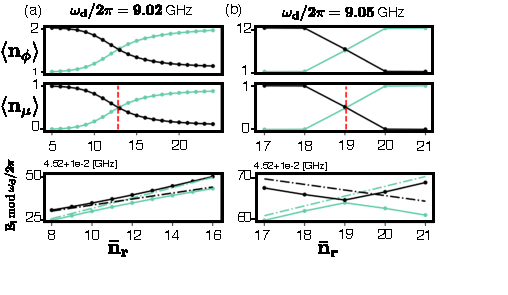
\includegraphics[width=\linewidth]{Figures/Floquet_011.pdf}
    \caption{Examples of p-MIST using transitions \textbf{(a)} $8$ and \textbf{(b)} $9$ from Table~\ref{tab:p-MIST} involving the $\ket{\tilde{1},\tilde{0}}$ state, with maximum overlap to the un-hybridized state $\ket{1}_\phi\otimes\ket{0}_{\mu=2}$. \textbf{Top row:} Qubit mode average occupation $\braket{n_\phi}$. \textbf{Middle row:} Parasitic mode average occupation $\braket{n_\mu}$. \textbf{Bottom row:} Stark-shifted eigen-energies (dashed) from first-order perturbative calculations, and quasi-energies (solid) from Floquet simulations showing avoided crossings. Plots are extracted from numerical data used in Fig.~\ref{fig:Floquet}. The data points are connected by lines for visual aid.}
    \label{fig:011}
\end{figure}

For further insights, we now examine in more detail how quasienergies and excitation numbers change as a function of drive power when we pass through an avoided crossing associated with a p-MIST process. Figs.~\ref{fig:011}(a,b) show explicitly how average qubit and parasitic mode excitation numbers change as a function of drive powers $\propto \bar n_r$ for fixed drive frequency corresponding to $8,9$ (respectively) in Table~\ref{tab:p-MIST}.  Both these transitions involve starting in the qubit's first excited state (i.e. branches associated with the undriven state $\ket{\tilde{1},\tilde{0}}$). The simultaneous exchange of population in the qubit mode $\phi$, shown in the top panels, and the parasitic mode $\mu=2$, shown in the middle panels, confirms that the transitions are indeed p-MIST. 

The bottom panel of Fig.~\ref{fig:011} shows the corresponding behavior of the branch quasi-energies as a function of drive power, for the same drive parameters.  We plot both quasi-energies coming from the Floquet calculations, as well as the predictions of a perturbative calculation including drive-induced Stark shifts (see App.~\ref{app:stark-shift} for details). For Fig.~\ref{fig:011}, the perturbative calculations do a good job of showing that there will be a crossing of energies, very near where an avoided crossing is seen in the Floquet calculations; this suggests that a simple picture of the crossings is possible. The Floquet calculations also clearly show an avoided crossing. Note that these transitions occur at relatively modest average readout cavity photon numbers $\bar n_r=11,19$. 


\subsection{Transition probability}\label{sec:LZ}
\begin{figure}[t]
    \centering
    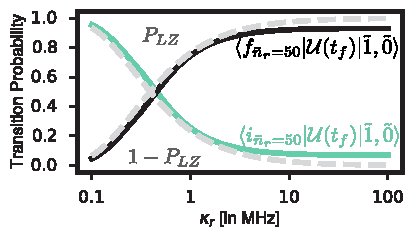
\includegraphics[width=\linewidth]{Figures/LZ.pdf}
    \caption{
    {\bf p-MIST transition probabilities as a function of readout cavity ring-up rate.}
    We plot the probabilities for adiabatic (green) and diabatic (black) transitions for a time-dependent ring-up of the average cavity photon number from $\bar{n}_r = 0$ to $\bar{n}_r = 50$, for different choices of the cavity damping rate $\kappa_r$ which controls the speed of the sweep (see text).  We start the system in the qubit's first excited state $\ket{\tilde{1},\tilde{0}}$.  The drive frequency is $\omega_d/2\pi=9.05 \ \mathrm{GHz}$, corresponding to the crossing shown in in Fig.~\ref{fig:011}(b).
    Here, $\ket{f_{\bar n_r=50}}$ and $\ket{i_{\bar n_r=50}}$ are the final states in the end of branch analyses for $\ket{\tilde{2},\tilde{1}}$ and $\ket{\tilde{1},\tilde{0}}$, respectively. The time-evolution operator is denoted by \singh{$ \hat{\mathcal{U}}(t_f)=\mathcal{T}\exp\big(-i\int^{t_f}_{0} \hat H_{s.c.}(t)dt\big)$ where $\mathcal{T}$} indicates time-ordering and $t_f=10/\kappa_r$. The adiabatic (green) curve corresponds to an unwanted p-MIST transition.  We also plot the predictions of the Floquet branch analysis combined with a Landau Zener approximation for the probabilities (grey), which are in excellent agreement over a wide range of $\kappa_r$.}
    \label{fig:LZ}
\end{figure}

Our Floquet branch analysis gives strong evidence that MIST and p-MIST transitions will occur during the ring-up of the resonant during a readout pulse.  Here, we validate this approach by focusing on a specific transition, and showing (via explicit time-dependent simulations) that it does indeed occur as predicted.  We also show that this full-time-domain simulation is in agreement with a Landau-Zener analysis that takes as inputs the result of the Floquet branch analysis.    

We focus on the p-MIST transition shown in Fig.~\ref{fig:011}(b), which corresponds to a fairly large avoided crossing energy of $\Delta_{ac}=0.66$ MHz. We will perform a full time-dependent simulation of $\hat H_{s.c.}$ in Eq.~\ref{eq:drive_Ham}, using time-dependent drive powers that are determined by a time-dependent average readout cavity photon number having the form:
\begin{align}
    \bar n_r(t)&:\bar n_r(1-e^{-\kappa_r t/2})^2.\label{eq:LZ-n}
\end{align}
This corresponds to the ring-up of a resonantly driven readout cavity with a damping rate $\kappa_r$~\cite{khezri2023measurement,dumas2024unified,cohen2023reminiscence}.  

To calculate transition probabilities in this full-time-dependent simulation, we start the system in the dressed state 
$\ket{\tilde{1},\tilde{0}}$, evolve under $\hat{H}_{s.c.}(t)$ from a time $t=0$ to $t = 10 / \kappa_r$, and then compute the overlap of this state with the Floquet branches of the two states $\ket{i}=\ket{\tilde{1},\tilde{0}}$ and $\ket{f}=\ket{\tilde{2},\tilde{1}}$ associated with our predicted transition.  We then repeat this calculation for different choices of $\kappa_r$, examining how the transition probabilities vary, with the results shown in Fig.~\ref{fig:LZ}. 
As expected, the probability of remaining adiabatic (green curve) decreases as one increases $\kappa_r$.  Note here that at large $\kappa_r$, adiabatic evolution corresponds to a detrimental p-MIST transition having occurred. The most likely final state $\ket{\tilde{2}, \tilde{1}}$ in this transition has an extra qubit and parasitic mode excitation compared to the initial state $\ket{\tilde{1}, \tilde{0}}$.  


The above probabilities are in very good agreement with the predictions of our Floquet branch analysis combined with a Landau-Zener approximation to the probability of a non-adiabatic transition (used here in a fashion similar to Ref.~\cite{ikeda2022floquet}, see App.~\ref{app:LZ}).  These probabilities ($P_{\mathrm{LZ}}$) are shown in grey in Fig.~\ref{fig:LZ}.   Similar to the transmon case in Ref.~\cite{dumas2024unified} we see agreement for most of the values of $\kappa_r$ between the time-domain simulations and our Landau-Zener calculations using the Floquet quasi-energies. 
\sh{However, for large $\kappa_r\rightarrow \infty$, we observe disagreement on the order of $~\sim\ 10$\%, which we attribute to the complexity of our two-mode system which is very likely to not be explained by the simple picture presented by the Landau Zener physics of a two-level system. In fact, it is surprising that despite this complexity we find such good agreement for small $\kappa$ values.}




\subsection{Post-readout qubit dephasing}\label{sec:dephasing}

The new p-MIST processes we identify here can also potentially create errors \textit{after} the readout pulse is complete, as they lead to a new dephasing channel.  A p-MIST process results in a JJA parasitic mode having a residual excitation post readout.  As there is a non-zero dispersive coupling 
$\chi_{\phi\mu}$ between these modes and the qubit, and as these modes are believed to have relatively large internal quality factors $Q\sim 10^{4}$~\cite{masluk_microwave_2012, masluk2013reducing}, this will lead to the qubit acquiring a random phase (tied to the random time at which the parasitic mode relaxes).  Below, we show master equation simulation results which quantify the
scale of phase errors that would result from such processes. 

\begin{figure}[htb]
    \centering
    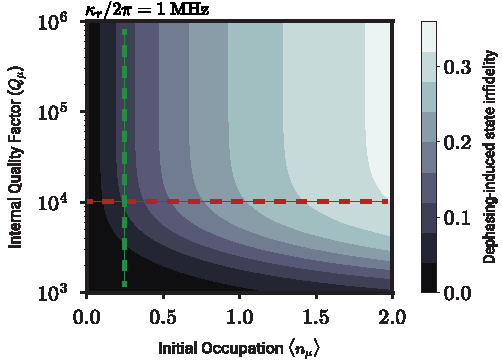
\includegraphics[width=\linewidth]{Figures/dephasing.pdf}
    \caption{Dephasing error probability due to random decay of an excited parasitic mode with occupation $\braket{n_\mu}$, after p-MIST, for various internal parasitic quality factor $Q_\mu$. The horizontal red line shows the quality factor quoted in~\cite{masluk_microwave_2012}. The green line shows the dephasing error probability for transition $9$ for various quality factors at $\kappa_r/2\pi=1 \ \mathrm{MHz}$ (see Figs.~\ref{fig:011}(b) and~\ref{fig:LZ}).}
    \label{fig:dephasing}
\end{figure}

For concreteness, we consider a readout pulse with a frequency corresponding to the p-MIST transition labeled $9$ in Fig.~\ref{fig:011}(b)), and for a cavity damping rate $\kappa_r/2\pi=1 \ \mathrm{MHz}$ (which determines the ring-up of the cavity to the maximum drive powers given by $\bar n_r=50$). 
For these parameters, our previous simulations and Landau-Zener analysis suggest that at the end of the readout pulse, the parasitic mode will have an average non-zero excitation $\braket{n_\mu}=0.25$.  In fact, for many transitions this population can be as high as $\braket{n_\mu}=2.0$ as shown in Table~\ref{tab:p-MIST}. We now ask how the decay of such population will dephase the fluxonium (assuming it is prepared after readout in the state $\ket{+}=\frac{\ket{0}_\phi+\ket{1}_\phi}{\sqrt{2}}$).  

A simple master equation simulation illustrates the resulting qubit dephasing due to this mechanism.  We investigate a reduced system of the parasitic mode $\mu=2$ and the fluxonium qubit (modeled as a two level system), interacting under the dispersive Hamiltonian $\hat H_\theta/\hbar=\chi_{\phi\mu} \hat a_\mu^\dagger \hat a_\mu \sigma_z$, and with a loss dissipator having collapse operator $\sqrt{\kappa_\mu}\hat a_\mu$, describing the parasitic mode internal loss.  We start the system in a product state, where the parasitic mode has some initial non-zero occupation, and the qubit is in the pure state $\ket{+}$. 
We let the system evolve for a time $T_f=10/\kappa_\mu$ long enough to allow the parasitic mode to relax, and then compute the fidelity of the final qubit state with the initial state $\ket{+}$, defining the error probability be the corresponding infidelity.  
This quantity is plotted in Fig.~\ref{fig:dephasing}, both as a function of the initial parasitic mode occupancy $\braket{n_\mu}$ and its internal quality factor $Q_\mu$. \singh{Here, we initialize the parasitic mode in a coherent state $\ket{\alpha}$ such that $|\alpha|^2=\braket{n_\mu}.$}  We find that for an internal quality factor $Q_\mu$ of $10^{4}$, an initial population of $\braket{n_\mu}=0.25$ in the parasitic mode introduces a dephasing error probability $\epsilon \sim 0.05$, which is already past the threshold of the surface code~\cite{fowler2012surface}. The explicit time-dependent simulations shown in Fig.~\ref{fig:011} indicate that using a realistic readout power of $\sim 10$ photons, the final post-readout parasitic mode population is $\braket{n_\mu}\sim 0.25$.  This population would already be enough to lead to a significant post-readout dephasing effect. 


%%%%%%%%%%%%%%%
\section{Effects of Circuit Modifications on p-MIST}\label{sec:expressions}
The p-MIST processes could actually be mitigated in various ways. Let's explore how adjusting the qubit frequency, readout resonator frequency, and parasitic mode frequencies, could help suppress unwanted transitions. We rely on derivations in Ref.~\cite{viola2015collective} for the circuit in Fig.~\ref{fig:meas_circuit}, as well as generalizations introduced in App.~\ref{app:alt_circuits}.



\subsection{Coupling Strengths} \label{sec:coupling}

Fig.~\ref{fig:coupling-Floquet} identifies the main culprit behind p-MIST as the fluxonium-parasitic-mode coupling, $g_{\phi \mu}$. We compare the results of Floquet branch analyses for the initial state $|\tilde{1}, \tilde{0}\rangle$ under different coupling conditions, drive frequencies, and amplitudes. Fig.~\ref{fig:coupling-Floquet}(a), reproduces as a reference the simulation results for our previous choice of coupling strengths $g_{\phi\mu}$ and $g_{\mu r}$. In contrast, Fig.~\ref{fig:coupling-Floquet}(b) shows the same simulation but with $g_{\phi \mu}$ set to zero. We observe that a non-negligible $g_{\phi\mu}$ is the main reason for p-MIST effects. This is evident from the absence of parasitic transitions $(8,9)$ in the top panel, and no streak or sharp change in color indicating parasitic mode excitations in the bottom panel:  for $g_{\phi \mu}=0$ the parasitic mode population always remains below $\braket{n_\mu}=10^{-4}$. 

Further, Fig.~\ref{fig:coupling-Floquet}(c) shows that turning the parasitic-readout coupling to zero shows no reduction in p-MIST. Thus, we can conclude that the qubit-readout coupling $g_{\phi r}$ alone does not cause significant transitions or p-MIST processes without $g_{\phi \mu}$. Therefore, reducing the coupling strength $g_{\phi \mu}$ is a potential path to reducing the likelihood of p-MIST processes. 
\begin{figure}[t]
    \centering
    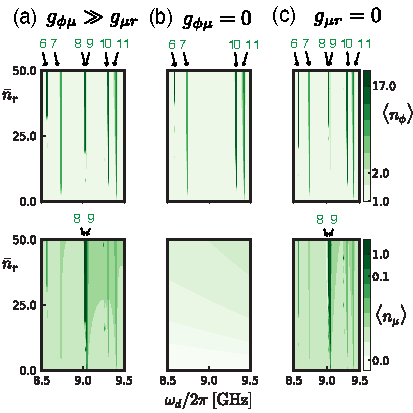
\includegraphics[width=\linewidth]{Figures/Floquet_coupling.pdf}
    \caption{
    {\bf Sensitivity of p-MIST processes to parasitic mode coupling strengths.} Panels show the result of Floquet branch analyses for the circuit parameters in Table~\ref{tab:circuit_params}. MIST processes observed in Fig.~\ref{fig:Floquet} are labeled with numbers and indicated with arrows. \textbf{(a)} All parameters the same as Fig.~\ref{fig:Floquet}(b). \textbf{(b)} Same, except now we set the parasitic mode to qubit coupling $g_{\phi \mu}$ to zero.  Note that all p-MIST features are now gone.  \textbf{(c)} Same as (a), but we now set the parasitic mode to readout resonator coupling $g_{\mu r}$ to zero.  As with previous Floquet branch analysis plots, color scales use a log scale scale to make transitions more visible.}
    \label{fig:coupling-Floquet}
\end{figure}

Next, we analyze the dependence of these coupling strengths on circuit and readout parameters. As discussed, only even-index parasitic modes have a non-zero coupling to the qubit~\cite{viola2015collective} (see derivation in App.~\ref{app:alt_circuits}). The coupling strength $g_{\phi \mu}$ between an even parasitic mode and the qubit is given by
\begin{align}
\frac{g_{\phi\mu}}{2\pi}&=\frac{4}{\sqrt{2N}} \frac{\tilde{E}^\phi_c\tilde{E}^e_{c,\mu}c_\mu}{E_{g,j}s_\mu^2}     \cdot {N_\phi}_{\mathrm{ZPF}} \cdot {N_\mu}_{\mathrm{ZPF}},
\end{align}
where $c_\mu=\cos{\frac{\pi\mu}{2N}},s_\mu = \sin \frac{\pi \mu}{2N}.\tilde{E}_c^\phi,\tilde{E}^e_{c,\mu} $ are the qubit and even parasitic mode charging energies, respectively, and $N_{\phi/\mu,\mathrm{ZPF}}$ are the zero-point fluctuation values for the qubit and parasitic modes. $\tilde{E}_c^\phi,N_{\phi/\mu,\mathrm{ZPF}}$ are given in Apps.~\ref{app:coupling}, and
\begin{align}
E_{c,\mu}^e&=\Big[\frac{1}{E_{C_j}}+\frac{1}{4E_{g,j}s_\mu^2}\Big]^{-1}.\label{eq:parasitic}
\end{align}
%\singh{where $s_\mu = \sin (\frac{\pi \mu}{2N})$.} 
All the other variables represent independent quantities listed in Table~\ref{tab:circuit_params}. 

We see that  suppressing the parasitic capacitance to ground near the junction array suppresses the qubit-parasitic coupling $g_{\phi\mu}$. However, this is constrained by practical limitations to order $\mathcal{O}(0.1) \ \mathrm{fF}$  per junction. The parasitic modes with the strongest coupling to the qubit have $\mu\ll N$. The large $N$, small $\mu$ limit with $c_\mu\approx 1$ yields
\begin{align}
    \tilde{E}^e_{c,\mu}\approx 4E_{g,j}s_\mu^2, \quad \tilde{E}^\phi_c\propto \frac{1}{N^2}\implies g_{\phi\mu}\propto \frac{1}{N^{5/2}}.\label{eq:dep1}
\end{align}
These dependencies are plotted in Fig.~\ref{fig:circuit_comp} of App.~\ref{app:coupling}. We find that the coupling strength \textit{decreases} with the number of junctions $N$, however, a limit to this increase may be set by the requirement of a constant inductance $E_L=E_{J_j}/N$ (see App.~\ref{app:coupling}). 
%\AC{I wonder if we should drop this discussion, as it seems a bit inconclusive.  On the one hand we argue large $N$ is good, but then we argue that you can't make it that big, and that you might run into trouble by making parasitic mode frequencies too small. If nothing else, can we just reduce the discussion here to a sentence or two?  Just say that large N in principle is good, but there is a limit to this strategy (e.g. qubit EL needs to stay at its target value).  }




\subsection{Mode Frequencies}\label{mode-frequencies}

An alternate strategy is to tailor the circuit so that the resonance conditions required for p-MIST are never realized. We can estimate these conditions by identifying energy-conserving processes, where $x$ drive photons are converted into a transition with an energy difference $\tilde{\Delta}_{if,y}$ in the hybridized eigenspace of the fluxonium and parasitic mode $\mu=2$. Here, $\tilde{\Delta}_{if,y}$ is the transition energy between levels $\ket{\tilde{i},\tilde{m}}$ and $\ket{\tilde{f},\tilde{n}}$ such that $|m-n|=y$. 
%In the disjoint Hilbert space, 
This equation can also be interpreted as a process where $x$ readout photons convert into $y$ parasitic mode photons and a fluxonium excitation $\ket{i}_\phi \leftrightarrow \ket{f}_\phi$ such that $\Delta_{if}=\hbar|\omega_f-\omega_i|$. To guide intuition for understanding the spectrum of resonance conditions, we plot such energy-conserving processes in Fig.~\ref{fig:trans_prof} that involve the parasitic mode $\mu=2$.
We plot all processes that are {\it approximately} energy conserving within a window $\epsilon$, i.e.~that satisfy:
%that satisfies $|x\omega_r-\tilde{\Delta}_{if,y}/\hbar|\le \epsilon$ which, in the disjoint Hilbert space corresponds to,
\begin{align}
\left(
    |x\omega_r-\tilde{\Delta}_{if,y}/\hbar| = 
|x\omega_r-y\omega_\mu-\Delta_{if}/\hbar| \right) \le \epsilon.
\label{eq:En_cons}
\end{align}
We take a fairly liberal value of $\epsilon / 25$ , to make sure we identify processes that could conceivably become resonant once Stark shifts due to the readout drive are accounted for (see App.~\ref{app:stark-shift} for details).

\begin{figure}[t]
    \centering
    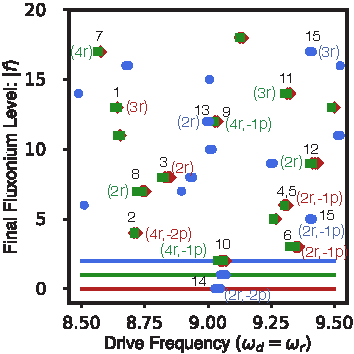
\includegraphics[width=\linewidth]{Figures/Trans_.pdf}
    \caption{Energy conserving processes $\ket{\tilde{i},\tilde{0}}\leftrightarrow\ket{\tilde{f},\tilde{y}}$ for Eq.~\ref{eq:En_cons} with $x\le 4, y\le 2, f\le 20$ and $i=0$ (red diamonds), $i=1$ (green squares), $i=2$ (blue circles). The horizontal lines indicate the initial state $i$ for visual aid. Labels in black correspond to transition $\#$ listed in Table~\ref{tab:p-MIST}. The colored labels correspond to the disjoint subspaces for simplified representation but the energy conservation uses the eigen-energies of the hybridized eigenstates of $H_{0}$ (see Eq.~\ref{eq:bare_ham}). For example, the green label ($4 \mathrm{r},-1 \mathrm{p}$), for transition $8$ of Table~\ref{tab:p-MIST}, shows the number of readout photons absorbed ($4$) and the number of parasitic mode ($\mu=2$) photons emitted ($1$) in the process. The faded points are weaker transitions not captured in the Floquet simulations. 
}
    \label{fig:trans_prof}
\end{figure}

Fig.~\ref{fig:trans_prof} depicts all four-photon processes that occur with approximate energy conservation, for drive frequencies within our target range, and when starting in one of the four lowest fluxonium levels. The results from Floquet simulations are  shown in solid dots and labeled in black (see Sec.~\ref{sec:MIST}), while the processes not identified in the simulation are faded. Note that there are downward transitions from $\ket{2}_\phi$ (blue dots) to the states $\ket{1}_\phi$ (green line) and $\ket{0}_\phi$ (red line) in the fluxonium subspace in the presence of parasitic modes. An example is captured by transition $14$ of Table~\ref{tab:circuit_params}. 

The parenthesized labels in color denote the number of readout photons ($x \mathrm{r}$) and parasitic mode photons ($y\mathrm{p}$) required for the transition in the fluxonium subspace, where a positive index denotes absorption/de-excitation while a negative index denotes emission/excitation. For example, transition $2$ corresponds to the emission of four readout photons, which are converted into two parasitic mode photons, absorbed by the mode $\mu=2$, as well as an excitation from $\ket{0}_\phi$ to $\ket{4}_\phi$ in the fluxonium subspace. 

Intuitively, many readout photons are required to bridge a large energy gap between the readout frequency and parasitic mode frequency. As this gap increases, the likelihood of p-MIST processes decrease. We verify this intuition
by considering the dependence on both the parasitic mode frequency and drive frequency in what follows.  


\paragraph{Parasitic Mode Frequency:}
An approach towards mitigating p-MIST processes is to adjust $\omega_\mu$ so that $\omega_\mu \gg\omega_r$ for $\mu=2$, requiring more readout photons to be absorbed in p-MIST processes and therefore reducing p-MIST transition rates. The dependence of the parasitic mode frequencies for even $\mu$ is
\begin{align}
    \frac{\omega_\mu^e}{2\pi}&=\sqrt{8E_{c,\mu}^e E_{J_j}}
\end{align}
 See Eq.~\ref{eq:parasitic} for $E_{c,\mu}^e$ and Table~\ref{tab:circuit_params} for $E_{J_j}$. Again, we focus on large $N$ and small $\mu$ limit to focus on parasitic modes with the strongest coupling to the qubit. From derivations in Ref.~\cite{viola2015collective} it is clear that parasitic frequency decreases with increase in junction count and 
 parasitic ground capacitance. Thus, decreasing parasitic ground capacitance decreases both parasitic frequency and qubit-parasitic coupling. Increasing $N$ on the other hand is only favorable for reducing the coupling strength while decreasing the gap between the between $\omega_d$ and $\omega_\mu$. The impact of decreasing $N$ to increase this gap would require consideration of nonlinear corrections as well as fixed inductance, thus, making these changes difficult in practice~\cite{viola2015collective}. 

\paragraph{Drive Frequency ($\omega_d$):} If, on the other hand, readout ($\omega_d \ll \omega_{\mu = 2}$), a large readout photon number $x$ would be needed while having a similar impact. We give the Floquet figure corresponding to a low-frequency readout regime in Fig.~\ref{fig:Flo_low} which shows higher parasitic mode populations compared to our previous case in Fig.~\ref{fig:Floquet}. The p-MIST effects can be explained by examining the increased density of resonances when $\omega_d/2\pi \approx 6 \ \mathrm{GHz}$. Note that this frequency is approximately the fluxonium plasma frequency $\omega_{12}/2\pi$ and is also half the parasitic mode $\mu=2$ frequency. This introduces multiple frequency collisions, which cause the various transitions observed in the figure. This logic already indicates that $5.5-6 \ \mathrm{GHz}$~\footnote{Further lower $\omega_d$ for readout is not favorable due to thermal heating of the readout resonator leading to photon-shot-noise induced dephasing of the qubit, and hence not analyzed in this work. } would be a bad range of frequencies for the current choice of parameters. Formal transition probability calculations, same as Sec.~\ref{sec:LZ}, will be required to predict the how detrimental these effects can be. However, the energy conservation indicates that in spite of the increase in the number of p-MIST effects, such transitions will be higher-order processes (large $x$) which will not take place unless $\bar n_r$ is extremely large.  

\begin{figure}[t]
    \centering
    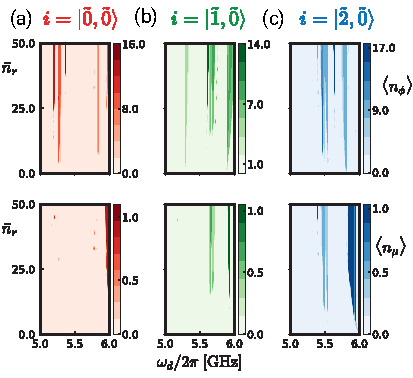
\includegraphics[width=\linewidth]{Figures/Floquet_low.pdf}
    \caption{Floquet simulations at lower readout frequencies using circuit parameters quoted in Tables~\ref{tab:circuit_params} and~\ref{tab:readout_params} for branch analysis starting in the dressed hybridized eigenstate $i=\ket{\tilde{k},\tilde{0}}$, with maximum overlap to the un-hybridized states $\ket{k}_\phi\otimes\ket{0}_{\mu=2}$. The figures are plotted in linear scale, unlike Fig.~\ref{fig:Floquet}, making any streak due to significantly weaker transitions unnoticeable.}
    \label{fig:Flo_low}
\end{figure}

A high-frequency readout $(\omega_d\gg \omega_{\mu=N-1})$ case requires a large Hilbert space and is beyond the scope of this work~\footnote{If  $\omega_d\gg \omega_{\mu=N-1}$, a dominating transition mechanism for p-MIST would correspond to an excitation of a strongly coupled, low-frequency parasitic mode (i.e., $\mu=\{2,4,6\}$) to a large photon number $y$, leaving just enough energy to produce excitation to some state $f$ in the fluxonium subspace of significant charge matrix elements (see Fig.~\ref{charge-matrix}). However such large excitations in the parasitic modes would occur with lower probability, because of the high photon number $y$ involved in the transition.}. 
% \AC{Can we possibly make the discussion in parts (a) and (b) more succinct?  There is a lot of detail here, fear we will lose the reader.  If there isn't a clear message or recommendation, might be best not to have a long discussion.}


\subsection{Alternative Circuit Parameters}\label{Will_circuit}

Our analysis of p-MIST so far has focused on systems where the fluxonium qubit frequency is $\omega_{01} / 2 \pi \sim 30$ MHz.  
Here, we consider how these processes change when one uses a larger qubit frequency $\omega_{01}/2\pi~\sim 300 \ \mathrm{MHz}$, as was recently realized in the experiment of Ref.~\cite{ding_high-fidelity_2023} (see App.~\ref{app:alt_circuit1} for full circuit parameters). 
%In the previous sections, we considered a fluxonium qubit frequency of  $\sim 30 \ \mathrm{MHz}$. To extend our results to other experiments, we consider these  circuit in Fig.~\ref{fig:meas_circuit}(a) with a different set of parameters inspired by Ref.~\cite{ding_high-fidelity_2023} and 
%We analyze p-MIST processes in setup where 
%$\omega_{01}/2\pi~\sim 300 \ \mathrm{MHz}$ 
The parasitic mode frequency of the $\mu=2$ mode is $\omega_{\mu=2}/2\pi=15.50 \ \mathrm{GHz}$. The coupling strengths are:  $g_{\phi r}/2\pi=37 \ \mathrm{MHz}$, $g_{\phi\mu}/2\pi=216 \ \mathrm{MHz}$, $g_{\mu r}/2\pi=6 \ \mathrm{MHz}$. The plasma frequency is $\omega_{12}/2\pi=5.40 \ \mathrm{GHz}$. % Importantly, here we only plot results for $\ket{\tilde{0},\tilde{0}}$ and $\ket{\tilde{1},\tilde{0}}$ because given Ref.~\cite{ding_high-fidelity_2023} uses only the first two levels for readout as well as computation. 
The assumptions for numerical modeling are the same as previous Floquet simulations as discussed in App.~\ref{app:numerics}. Even though the coupling strengths for these circuit parameters are similar to our previous parameter set in Table~\ref{tab:readout_params}, since the $\mu=2$ parasitic mode mode is larger by about $4 \ \mathrm{GHz}$, we expect fewer p-MIST processes for the drive frequency range analyzed in Fig.~\ref{fig:Floquet}. 

\begin{figure}[t]
    \centering
    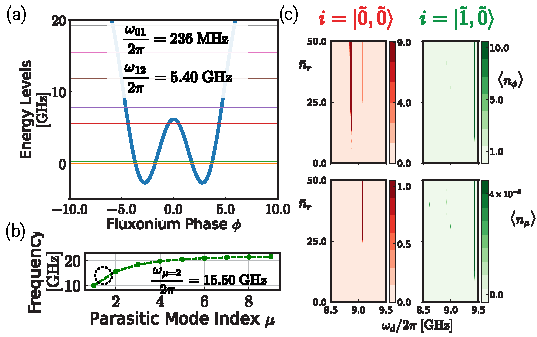
\includegraphics[width=\linewidth]{Figures/Floquet_Will.pdf}
    \caption{Floquet analysis with alternate JJA fluxonium parameters inspired by Ref.~\cite{ding_high-fidelity_2023}. \textbf{(a)} Fluxonium energy spectrum. \textbf{(b)} Parasitic mode frequencies. \textbf{(c)} Floquet simulations for the branch analysis of the computational states. Circuit parameters for this circuit are discussed in Sec.~\ref{Will_circuit} and App.~\ref{app:alt_circuit1}. The Floquet figures are plotted in linear scale unlike Fig.~\ref{fig:Floquet}, making any streak due to significantly weaker transitions unnoticeable.}
    \label{fig:Floquet1}
\end{figure}

Fig.~\ref{fig:Floquet1} shows that indeed, p-MIST effects are comparatively less likely for this alternate circuit. The single p-MIST process observed in the Floquet profile $\ket{\tilde{0},\tilde{0}}\leftrightarrow\ket{\tilde{4},\tilde{1}}$ occurs at $\bar n_r=25$ and has the quasi-energy gap of $\Delta_{ac}=0.13 \ \mathrm{MHz}$ at the avoided crossing. The quasienergy gap at the avoided crossing for this transition is $\Delta_{ac}=0.12$ MHz. The corresponding Landau-Zener probabilities and explicit transitions with quasienergies for the Floquet profile shown in Fig.~\ref{fig:Floquet1}(c) can be found in App.~\ref{app:alt_circuit1}. However, a detailed understanding of this Floquet profile, including rate calculations, is necessary to make proper claims about the target drive frequency regime inducing a favorably reduced number of MIST processes, and is left as future direction.


\section{Conclusion and Further Work}\label{sec:conclusion}
%%%%Summary/inferences&&&&&&

In this work, we have analyzed the impact of parasitic modes on driven JJA fluxonium qubits, showing that measurement-induced state transitions of a fluxonium qubit can occur via excitations of a parasitic mode of the JJA. These transitions occur at particular resonance conditions when the energy of several readout photons is equal to a small number of parasitic mode excitations and a fluxonium mode excitation.  We refer to these transitions as parasitic-mode-induced-state-transitions or p-MIST, inspired by the term MIST for measurement-induced-state transitions~\cite{sank2016measurement}. 

We find that p-MIST transitions can occur at meaningfully-high rates because of the strong coupling between  parasitic modes and the qubit. Consequently, it is possible to have qubit state transitions mediated via JJA internal mode iduring fluxonium readout, even at low average readout photon numbers and while using typical parameters that enable high fidelity, dispersive readout. We show that p-MIST does lower the onset of MIST processes to $\sim 10$ readout photons at certain drive frequencies. In addition, it has the potential to significantly dephase the qubit post-measurement, which could in turn limit the qubit gate fidelities required for quantum error correction, and ultimately the performance of a quantum processor. However, the coupling of the parasitic mode to the readout is still sufficiently weak such that, for the vast majority of readout frequencies, the JJA mode excitation population is negligible unless a p-MIST occurs. Therefore, these processes can be avoided via judicious choice of readout, junction array, and fluxonium parameters.
We analyze the trend in p-MIST for various drive frequencies, parasitic mode frequencies, coupling constants, and circuits with two different qubit frequencies equal to $\sim 30$ and $\sim 300 \ \mathrm{MHz}$. 

%alternatives
%Given the strong coupling between parasitic modes and fluxonium, these modes could even be used as the readout resonator for the fluxonium qubit. In this case, a Purcell filter would be needed to protect the qubit from radiative decay, while coupling the $\mu = 2$ parasitic mode to the Purcell filter and readout feed-line. This approach could help to alleviate the stringent capacitive loading constraints that plague the high-impedance fluxonium qubit. Alternative readout schemes like longitudinal readout or cloaking could also be explored with renewed motivation~\cite{reed_high-fidelity_2010, munoz-arias_qubit_2023, didier_fast_2015}.

We have presented a first analysis toward understanding the role of parasitic modes in the dispersive readout dynamics of a fluxonium circuit. Mitigating the parasitic mode excitations could involve careful selection of the readout resonator frequency, and varying junction energies along the array to localize parasitic modes, thereby altering the parasitic mode spectrum and reducing excitation probability. The circuit parameters used in this work correspond to a parasitic mode of the fluxonium's junction array. However, other modes with similar frequencies may also participate in the environment of the fluxonium. This may include, for example, confined package modes, slot line modes, and harmonics of coplanar waveguide resonators for readout. Our results show the significance of taking all such modes into consideration when driving many excitations into highly nonlinear circuits.  

\AC{End of Aash edits Nov. 11}



\section{Acknowledgments}
 We thank Akshay Koottandavida, Daniel K. Weiss, Connor Hann, Kyungjoo Noh, Simon Leiu and Vidul R. Joshi for fruitful discussions. We are grateful to Simone Severini, Bill Vass, Oskar Painter, Fernando Brand\~ao, Eric Chisholm, and AWS for supporting the quantum computing program. %SS acknowledges support from the Army Research Office (ARO) under Grant Number W911NF-23-1-0051 for the time she spent on this project at Yale. SS is grateful to Connor Hann for inviting her to pursue an internship program at AWS where this project started.
\appendix
\section{Single-Point Connections}\label{app:alt_circuits}
%Appendices for Sec 4
\begin{figure*}[htb]
    \centering
    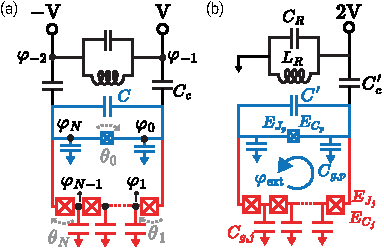
\includegraphics[width=\linewidth]{Supp_Fig/Circuit_choice.pdf}
    \caption{(a-c) Alternative readout circuits. (a) Parallel circuit ($H_1$), (b) Floating fluxonium ($H_2$), (c) Grounded fluxonium ($H_3$). Alternatives (b) and (c) require a single-point connection to the readout line $V$, unlike the parallel circuit in (a). We maintain the values for all circuit variables the same as used for the case of the parallel circuit in Fig.~\ref{fig:meas_circuit}. (d) Absolute values of the coefficients of coupling terms in the Hamiltonian (in GHz). We can see that the parasitic modes couple to the qubit stronger than the qubit couples to the readout. The parasitic mode coupling to the readout is very slightly weaker in $H_3$ compared to $H_1$, $H_2$. Need to add the flux variables in Figs.(a,b,c)}
    \label{fig:circuit_choice}
\end{figure*}

\begin{table}[htb]
    \begin{center}
    \begin{tabular}{|c |c| c |c| }
     \hline
     \textbf{Parameters} & \textbf{Variables} & \textbf{Values}\\ 
    \hline
    Phase-slip JJ capacitance &$C_p$ &$13.3$ fF\\ 
    \hline
    Differential capacitance &$C$ &$1.14$ fF\\ 
    \hline
    JJA capacitance energy&$C_j$&$26.2$ fF\\ 
    \hline
    JJA ground capacitance&$C_{g,j}$&$0.1 \ \mathrm{fF}$\\ 
    \hline
    Phase-slip ground capacitance&$C_{g,p}$&$10 \ \mathrm{fF}$\\ 
    \hline
    Coupling capacitance&$C_c$ &$1 \ \mathrm{fF}$\\ 
     \hline
      ZPF of the resonator/drive&$V_{\mathrm{ZPF}}$&$0.75$ GHz\\
     \hline
      ZPF of fluxonium charge operator&$N_{\phi,\mathrm{ZPF}}$&$0.36$\\
     \hline
      ZPF of parasitic charge operator&$N_{\mu=2,\mathrm{ZPF}}$&$1.58$\\
     \hline
    \end{tabular}
    \end{center}
    
    \caption{Capacitances and zero-point fluctuation (ZPF) values for the fluxonium readout circuit used in the main text.}
    \label{tab:params}
    \end{table}
The fluxonium readout circuit shown in Fig.~\ref{fig:meas_circuit} of main text can have several modifications, each of which may affect various performance metrics. Here, in Fig.~\ref{fig:circuit_choice}, we present two modifications to the parallel circuit, with different grounding options for the fluxonium while the readout resonator is \singh{grounded}. We will refer to these circuit choices as: $H_1$, parallel circuit in Fig.~\ref{fig:circuit_choice}(a) (same as Fig.~\ref{fig:meas_circuit}), $H_2$, floating fluxonium circuit in Fig.~\ref{fig:circuit_choice}(b), and $H_3$, grounded fluxonium circuit in Fig.~\ref{fig:circuit_choice}(c). We adjust the coupling capacitances (using $C_c'=5.06 \ \mathrm{fF},C_c''=4.12 \ \mathrm{fF}$ in Figs.~\ref{fig:circuit_choice}(b,c)) and the total capacitance of the phase slip junction (busing $C'=4.97 \ \mathrm{fF},C''=5.8 \ \mathrm{fF}$ in Fig.~\ref{fig:circuit_choice}(b,c)), as compared to the values for the parallel circuit given by Table~\ref{tab:params}. These modifications achieve the same qubit frequency $\omega_{01}/2\pi$, plasmon frequency $\omega_{12}/2\pi$, qubit-readout coupling constant $g_{\phi \mu}$ and qubit-readout dispersive shift $\chi_{\phi r}$ for the three circuits as given by Table~\ref{tab:readout_params}. Under these choices, we find that the readout parameters affected by parasitic modes are roughly the same across all three circuits, given our assumptions of ordered array and no self-nonlinearity in parasitic modes. See Table~\ref{tab:parasitic_params} in App.~\ref{app:Hamiltonian} for details. 


We will now derive the Hamiltonians for the circuits in Figs.~\ref{fig:circuit_choice}(b,c) to be used in the next section for comparison. To do this, we follow the recipe given in Ref.~\cite{viola2015collective} for the parallel circuit shown in Fig.~\ref{fig:circuit_choice}(a) or Fig.~\ref{fig:meas_circuit}(a). Importantly, we will show that the symmetry in the parallel circuit which prevents any coupling with the lowest-frequency parasitic mode ($\mu=1$) is preserved in all three circuits, absence of which would have changed the Floquet landscape across the three circuits significantly. 


\subsection{Floating Fluxonium Circuit}
The Lagrangian corresponding to these circuits is a combination of the Lagrangians $\mathcal{L}_g$ from the phase-slip junction (comprising of the junction with $E_J/E_C\sim 5-8$ and the capacitor $C$), $\mathcal{L}_{g}$ from the ground capacitances, $\mathcal{L}_{R}$ from the readout resonator and $\mathcal{L}_c$ due to the coupling capacitances $C_c$ and the external voltage $V$. We mark the flux points across JJA using $\varphi_0$ and $\varphi_{N}$ in Figs.~\ref{fig:circuit_choice}(b,c). We start with an in-homogenous junction array and will use the assumption of ordered junction later in the derivation. The flux variables and voltage variables in the circuit are denoted by $\varphi_n=2\pi\Phi_n/\Phi_0$ and $\dot{\varphi}_n=2\pi V_n/\Phi_0$, respectively, where $\Phi_0=h/2e$ is the superconducting flux quantum. We will use subscripts $j, p$ for JJA and the phase-slip junction coordinates, respectively. Transforming the Lagrangian in Ref.~\cite{viola2015collective}, the following terms will remain the same in the case of floating fluxonium circuit:
\sh{check for the derivation to include $\hbar =1$ and not h=1}

\begin{align}
    \mathcal{L}&=\mathcal{L}_{phase-slip}+\mathcal{L}_{JJA}+\mathcal{L}_{g}+\mathcal{L}_{R}+\mathcal{L}_{C}\\
    \mathcal{L}_{phase-slip}&=\frac{(\dot{\varphi}_N-\dot{\varphi}_0)^2}{16E_{C'}}-E_{J_p}\cos(\varphi_0-\varphi_{N}+\varphi_\mathrm{ext})\\
    \mathcal{L}_{JJA}&=\sum_{n=1}^N\frac{(\dot{\varphi}_n-\dot{\varphi}_{n-1})^2}{16E^{n}_{C_j}}-E^{n}_{J_j}\cos(\varphi_n-\varphi_{n-1})\\
    \mathcal{L}_{R}&=\frac{\dot{\varphi}_{-}^2}{16E_{{R}}}-\frac{\varphi_{-}^2}{16E_{R}}\\
    \mathcal{L}_{g}&=\sum_{i=0}^{N} \frac{\dot{\varphi_n}^2}{16E_{g_i}}\label{eq:float-float}
  \end{align}
The change in this Lagrangian is primarily due to the fewer coupling capacitances such that,
\begin{align}
\mathcal{L}_{c}&=\frac{(\dot{\varphi}_{-1}-\dot{\varphi_0})^2}{16E_{c'}}=\frac{\dot{\varphi}^2_0}{16E_{c'}}+\frac{\dot{\varphi}^2_{-1}}{16E_{c'}}-\frac{\dot{\varphi}_0\dot{\varphi}_{-1}}{8E_{c'}}
\end{align}
Now, we define the guage-invariant phase difference quadratures 
\begin{align}
\varphi_m-\varphi_0=\sum_{l=1}^m\theta_l
\end{align}
and use the fluxoid quantization with an external flux $\varphi_{\mathrm{ext}}=\pi$.
\begin{align}
\\ \sum_{m=0}^N \theta_m+\varphi_\mathrm{ext}&=2\pi z,
\end{align}
where $z\in\mathbb{Z}$ is an arbitrary integer. Writing the lagrangian in this new basis yields the expression,
\begin{align}
    \dot{\varphi}_0=E_t\Big(\frac{\dot{\varphi}_{-1}}{E_{c'}}-\sum_{n=1}^N\sum_{m=n}^N\frac{\dot{\theta}_n}{E_{g_m}}\Big)
\end{align}
where 
\begin{align}
E_t=\Big(\frac{1}{E_{c'}}+\sum_{n=0}^N\frac{1}{E_{g_n}}\Big)^{-1}
\end{align}
is the total capacitive energy of the circuit due to the parasitic and coupling capacitances.

\begin{align}
\therefore     \mathcal{L}_g+\mathcal{L}_c&=\frac{\dot{\varphi}^2_{-1}}{16E_{c'}}\Big(1-\frac{E_t}{E_{c'}}\Big)+\sum_{n=1}^N\frac{\dot{\varphi}_{-1}\dot{\theta}_n}{E_{c'}}\Big(\sum_{i=n}^N\frac{E_t}{8E_{g_i}}\Big)\nonumber\\&\quad+\sum_{m=1}^N\sum_{n=1}^N\dot{\theta}_m\dot{\theta}_{n}\Big( \sum_{j=\text{max}\{m,n\}}^N\frac{1}{16E_{g_j}}\Big)\nonumber\\&\quad\quad
\times\Big(1-\sum_{i=\text{min}\{m,n\}}^N\frac{E_t}{E_g^i}\Big)
\end{align}
We simplify the Lagrangian $\mathcal{L}_g+\mathcal{L}_c$ as
\begin{align}
    &=\frac{\dot{\varphi}_{-1}eV}{8E_c}+\frac{\dot{\varphi}^2_{-1}}{16}\Big(\frac{1}{E_c}\Big(1-\frac{E_t}{E_c}\Big)+\frac{1}{E_c}\Big)\nonumber\\&+\sum_{n=1}^N\Big(\frac{\dot{\varphi}_{-1}\dot{\theta}_n}{E_c}\Big)(N-n+1)\frac{E_t}{8E_g}+\frac{(\dot{\varphi}_{-2})^2}{16E^4_{c}}\nonumber\\
&+\sum_{m=1}^N\sum_{n=1}^N\dot{\theta}_m\dot{\theta}_{n} \frac{(N-\text{max}\{m,n\}+1)\text{min}\{m,n\}E_t}{16E_g^2}
\end{align}
\paragraph{Assumptions.} 
The first line show that the contribution from the coupling capacitance comes only via the readout resonator mode. The second and third lines, on the other hand, show the terms which contribute to parasitic couplings via the the ground capacitance due to terms proportional to $\dot{\theta}_m\dot{\theta}_n$. Now, we will assume an ordered array such that
\begin{align*}
    C_{g_1}=...C_{g_{N-1}}=C_{g,j} \\
    C_{g_0}=C_{g_N}=C_{g,p} \\
    E_{J_1}=...=E_{J_N}=E_{J,j} \\
    C_{j_1}=...=C_{j_N}=C_{j} 
\end{align*}
\paragraph{Collective Modes.} 
Now, we will define the collective modes for the fluxonium circuit, $\{\phi,\xi_1,...,\xi_{N-1}\}$ such that 
\begin{align}
    \theta_m=\phi/N+\sum_\mu W_{\mu m}\xi_\mu,
\end{align}
and inversely,
\begin{align}
    \phi&=\sum_{m}\theta_m,\quad \xi_\mu=\sum_m W_{\mu m}\theta_m.
\end{align}
Here, $\phi$ is called the superinductance mode or the \emph{qubit} mode while $\xi_\mu$ denote the parasitic modes indexed by $\mu\in\{1,..,N-1\}$~\cite{ferguson2013symmetries}. The matrix $W$ is semi-orthogonal, with dimensions $(N-1)\times N$, and is given by $\sum_m W_{\mu m}W_{\nu m}=\delta_{\mu \nu}$. Its row sum is zero, $\sum_mW_{\mu m}=0$. Thus, the following choice
\begin{align}
    W_{\mu m}=\sqrt{\frac{2}{N}}\cos{\frac{\pi\mu(m-1/2)}{N}},
\end{align}
is observed in~\cite{ferguson2013symmetries} and later used in~\cite{viola2015collective} to derive the Hamiltonian for the parallel circuit.
The choice of these new variables highlights the collective modes describing the low-energy physics as illustrated in~\cite{catelani2011relaxation,koch2009charging,manucharyan2009fluxonium}. We can now split the combined Lagrangian $\mathcal{L}=\mathcal{T}-\mathcal{U}$ into kinteic energy $\mathcal{T}$ and potential energy $
\mathcal{U}$ terms in the basis of collective modes as, \sh{Here on, we need to remove terms due to Ec3 and Ec4, and also point out where the symmetry from the odd modes is coming from. We also need to separate Egj and Egp}
\begin{align}
\mathcal{T}=&\frac{\dot{\varphi}^2_{-1}}{16E_{c'}}\Big(1-\frac{E_t}{E_{c'}}\Big)+\frac{1}{E_{c'}}\Big(1-\frac{E_t}{E_{c'}}\Big)\nonumber\\
      &+\Big[\sum_{n=1}^N\Big(\frac{\dot{\varphi}_{-1}}{E_c}+\frac{\dot{\varphi}_{-2}}{E_c}\Big)\Big(\frac{E_t}{8E_c}+(N-n+1)\frac{E_t}{8E_g}\Big)\nonumber\\&\quad-\sum_{n=1}^N\frac{\dot{\varphi}_{-2}}{8E_c}\Big](\dot{\phi}/N+\sum_\mu W_{\mu n}\dot{\xi}_\mu)+\sum_{m=1}^N\sum_{n=1}^N(\dot{\phi}/N\nonumber\\
  &+\sum_\mu W_{\mu n}\dot{\xi}_\mu)(\dot{\phi}/N+\sum_\mu W_{\mu m}\dot{\xi}_\mu)\Big( (N-\text{max}\{m,n\}\nonumber\\&+1)\frac{1}{16E_g}+\frac{1}{16E_c}\Big)\Big(\text{min}\{m,n\}\frac{E_t}{E_g}+\frac{E_t}{E_c}\Big)\label{eq:kin-energy}\\
    \mathcal{U}&=-E_{J_p}\cos(\phi)-\frac{(\varphi_{-1}-\varphi_{-2})^2}{16E_{R}}\nonumber\\&\quad-\sum_{n=1}^NE_{J_j}\cos\Big(\phi/N+\sum_\mu W_{\mu n}\xi_\mu\Big)\label{eq:pot-energy}
\end{align}

\paragraph{Symmetries in the Lagrangian}
Simplifying the kinetic energy term from Eq.~\ref{eq:kin-energy}, recalling that $\sum_m W_{\mu m}=0$, and the semi-orthogonal matrix condition $\sum_m W_{\mu m}W_{\nu m}=\delta_{\mu\nu}$ yields
\begin{align}
\mathcal{T}&=-\frac{\dot{\varphi}_{-2}eV}{16E_{c'}}+\frac{\dot{\varphi}_{-1}eV}{16E_{c'}}-E_t\frac{\dot{\varphi}_{-1}\dot{\varphi}_{-2}}{16E_{c'}^2}\nonumber\\
    &+\frac{\dot{\varphi}^2_{-1}}{16}\Big(\frac{1}{E_c}\Big(1-\frac{E_t}{E_c}\Big)+\frac{1}{E_c}\Big)\\&+\frac{\dot{\varphi}^2_{-2}}{16}\Big(\frac{1}{E_c}+\frac{1}{E_c}\Big(1-\frac{E_t}{E_c}\Big)\Big)\nonumber\\&\quad+\frac{E_t}{8E_c^2}\dot{\varphi}_{-1}\dot{\phi}+\frac{E_t}{8E_c^2}\dot{\varphi}_{-2}\dot{\phi}\nonumber\\
      &+\Big[\sum_{n=1}^N\Big(\frac{\dot{\varphi}_{-1}}{E_c}+\frac{\dot{\varphi}_{-2}}{E_c}\Big)\Big(\frac{E_t}{8E_c}+(N-n+1)\frac{E_t}{8E_g}\Big)\nonumber\\&\quad-\sum_{n=1}^N\frac{\dot{\varphi}_{-2}}{8E_c}\Big](\dot{\phi}/N+\sum_\mu W_{\mu n}\dot{\xi}_\mu)\nonumber\\
    &\quad+\Big[(M_{00}+G_{00})\dot{\phi}^2+2\sum_{\mu}(M_{0\mu}+G_{0\mu})\dot{\phi}\dot{\xi_\mu}\nonumber\\&\quad+\sum_{\mu,\nu}(M_{\mu\nu}+G_{\mu\nu})\dot{\xi_\mu}\dot{\xi_\nu}\Big],    
    \end{align}
where the coefficients are given by
\begin{align}
    M_{00}&=\frac{1}{16E_{C'}}+\frac{1}{16NE_{C_j}},\quad M_{0\mu}=0,\quad    M_{\mu\nu}=\frac{\delta_{\mu\nu}}{16E_{C_j}}\\
    G_{00}&=\frac{1}{64E_t}\Big(1-\frac{E_t}{E_c}\Big)^2\Big[1-\frac{2}{3}\frac{N-1}{N}\Big]\\
    G_{0\mu}&=-\frac{c_\mu o_{\mu+1}}{16E_g\sqrt{2N}s_\mu^2}\Big(1-\frac{E_t}{E_c}\Big)\\
    G_{\mu\nu}&=\frac{1}{64E_gs_\mu^2}\Big[\delta_{\mu\nu}-\frac{E_t}{E_g}\frac{2c_\mu c_\nu o_\mu o_\nu}{N s_\nu^2}\Big].
\end{align}
\sh{Define c,o.}
The quantities $G_{00},G_{0\mu},G_{\mu\nu}$ contribute to the equations for coupling strengths while $M_{00},M_{\nu\nu}$ contribute to the charging energies of the qubit and parasitic modes, discussed in Sec.~\ref{sec:expressions}. Note that $G_{00}$ increases quadratically with a factor of $\Big(1-\frac{E_t}{E_c}\Big)$. Thus, $G_{0\mu}$ is different from the parallel circuit by a factor $\Big(1-\frac{E_t}{E_c}\Big)$. The last term, $G_{\mu\nu}$ same as the case of parallel circuit quoted in Ref.~\cite{viola2015collective} because it has no dependence on coupling capacitances.
\paragraph{Linear Approximation}
From here on, we define a sum over $m,n$ as running from $1$ to $N$, while the sum over $\mu,\nu$ runs from $1$ to $N-1$. Simplification to including only linear terms from Taylor expansion of the cosine ($\cos{x}\sim 1-\frac{x^2}{2}$) Eq.~\ref{eq:pot-energy} and using $\sum_{n}W_{\mu m}W_{\nu m}=\delta_{\mu\nu}$, yields (up to a constant term)
\allowdisplaybreaks{
\begin{align}
    \mathcal{U}&=E_{J_p}\cos(\phi)-\frac{(\varphi_{-1}-\varphi_{-2})^2}{16E_{R}}\nonumber\\&\quad+\frac{E_{J_j}}{2N}\phi^2+\frac{E_{J_j}}{2}\sum_{\mu}\xi_\mu^2\\
    &=E_{J_p}\cos(\phi)+\frac{E_{J_j}}{2N}\phi^2+\frac{E_{J_j}}{2}\sum_{\mu}\xi_\mu^2-\frac{\varphi_{-}^2}{16E_{R}},
    \end{align}
    }
where $\dot{\phi}_{-1}=-\dot{\phi}_{-2}=eV$
\sh{Need to remove eV in this derivation}

We can see that there is no choice of $\dot{\varphi}_{\pm}$ such that the parasitic coupling between the readout resonator and fluxonium can be canceled without eliminating the coupling between the qubit and readout resonator. Note that, $\frac{N+1}{E_g}=\frac{1}{E_g}-\frac{1}{E_c}$ \sh{weird!}, and thus, the coupling between the qubit and the readout is same as the parallel circuit if $E_g \ll E_c$ with a lower $N$. We drive the readout resonator, such that, $\dot{\varphi}_{-}\equiv 2eV$ (the sign of the voltage value has been changed because in this circuit $\varphi_{-1}$ will be connected to $V$ and not $-V$, just for simplicity).
\begin{align}
    \mathcal{L}&=\frac{\dot{\varphi}_{+}^2}{64E_c}\Big(2+\frac{(N+1)E_t}{E_g}\Big)+\frac{\dot{\varphi}_{+}eV}{16E_c}\Big(\frac{3}{2}+\frac{E_t}{E_c}\Big)\nonumber\\
    &\quad-\frac{(N+1)E_t}{32E_gE_c}\dot{\phi}eV+\frac{(N+1)E_t}{64E_gE_c}\dot{\phi}\dot{\varphi}_{+}\nonumber\\
    &\quad -\frac{E_t}{16E_gE_c} \sum_\mu\frac{c_\mu o_\mu}{\sqrt{2N}s_\mu^2}  \dot{\xi}_\mu eV\nonumber\\
    &\quad+\frac{E_t}{32E_gE_c} \sum_\mu\frac{c_\mu o_\mu}{\sqrt{2N}s_\mu^2}  \dot{\xi}_\mu\dot{\varphi}_{+}\mathcal{O}(e^2V^2)\nonumber\\
    &\quad+\Big[(M_{00}+G_{00})\dot{\phi}^2+2\sum_{\mu}(M_{0\mu}+G_{0\mu})\dot{\phi}\dot{\xi_\mu}\nonumber\\
    &\quad+\sum_{\mu,\nu}(M_{\mu\nu}+G_{\mu\nu})\dot{\xi_\mu}\dot{\xi_\nu}\Big]-\mathcal{U}
\end{align}
\sh{Correct the derivation in numerics and text to only use grounded resonator and then extend briefly to the floating case. We are ding so by eliminating all terms with $E_c^3, E_c^4$ and using $\dot \varphi_{-2}=0, \dot\varphi_{-1}=-2eV$. Thus, $\varphi_{+}=\varphi_{-}=-2eV$. So this point everything will be correct and we do not need to change the equations for Ec but only for Eg
} 
\begin{align}
    &=-\frac{(N+1)E_t}{16E_gE_c}\dot{\phi}eV-\frac{E_t}{8E_gE_c} \sum_\mu\frac{c_\mu o_\mu}{\sqrt{2N}s_\mu^2}  \dot{\xi}_\mu eV\nonumber\\
    &\quad+\Big[(M_{00}+G_{00})\dot{\phi}^2+2\sum_{\mu}(M_{0\mu}+G_{0\mu})\dot{\phi}\dot{\xi_\mu}\nonumber\\&\quad+\sum_{\mu,\nu}(M_{\mu\nu}+G_{\mu\nu})\dot{\xi_\mu}\dot{\xi_\nu}\Big]-\mathcal{U}
\end{align}
\paragraph{Hamiltonian:} 
We will now use Legendre transformation to obtain Hamiltonian variables,
\begin{align}
     p_{\phi}&=\frac{\partial \mathcal{L_K}_o}{\partial \dot{\phi}}=2(M_{00}+G_{00}) \dot{\phi}+\sum_{\mu}(M_{\mu 0}+G_{\mu 0})\dot{\xi}_{\mu}\nonumber\\
    &\quad-\frac{(N+1)E_t}{16E_gE_c}eV\\
    p_{\xi_\mu}&=\frac{\partial \mathcal{L_K}_o}{\partial \dot{\xi}_\mu}=(M_{0\mu}+G_{0\mu}) \dot{\phi}+2\sum_{\nu} (M_{\mu\nu}+G_{\mu\nu}) \dot{\xi}_\nu\nonumber\\
    &\quad-\frac{E_t}{8E_gE_c} \sum_\mu\frac{c_\mu o_\mu}{\sqrt{2N}s_\mu^2}eV
    \end{align}
\sh{define odd and even sectors and then check what is different here.}
    Here, the even and odd sectors are not decoupled due to the $eV$ term. The even and odd sectors can be diagonalized independently, such that a rotation on the odd sectors does not affect the even sectors. This is contrary to the case of Eq. 77 in~\cite{viola2015collective} where the rotation of odd sectors affects the even sectors. This is because in that case $G_{0\mu}$ was changed to being dependent on odd as well as even sectors. However, here, only the $\mathcal{L}_V$ term has changed. Thus, if the following condition is satisfied, 
\begin{align}
     \frac{\tilde{E}_{c}^{\phi}\tilde{E}_{c,j}^{e}c_i c_j}{32NE_g^2s_i^2 s_j^2}&<<1\implies \frac{4E_g\tilde{E}_{c}^{\phi}c_i c_j}{32NE_g^2s_i^2 }<<1\\
     \implies \frac{4\tilde{E}_{c}^{\phi}N}{8E_g \pi^2\mu\nu }&<<1\implies N<<8\pi^2\frac{E_g}{\tilde{E}_{c}^{\phi}},
 \end{align}
\sh{quote the N} we can carry out the exact same procedure as Ref.~\cite{viola2015collective} to simplify the inversion of matrix for the Legendre transformation and obtain the Hamiltonian as follows. Thus, we arrive at the following Hamiltonian
 \begin{align}
\quad H_2&= 4\bar{E}^\phi_cp_\phi^2+\sum_{\mu=1}^{N-1} 4\tilde{E}^{e/o}_{c,\mu}p_\mu^2\nonumber\\
    &\quad+2\sum_{\mu=1}^{N-1} \frac{\bar{E}^\phi_c\tilde{E}^{e/o}_{c,\mu}c_\mu o_{\mu+1}}{\sqrt{2N}E_gs_\mu^2} p_\phi p_\mu \nonumber\\
&\quad -\bar{E}_c^\phi p_\phi eV\Big[\frac{(N+1)E_t}{2E_gE_c}+\frac{E_t^2\tilde{E}_{c,\mu}^{e/o}}{8E_g^2E_c^2} \Big(\frac{c_\mu^2 o_\mu}{2Ns_\mu^4}\Big)\Big]\nonumber\\
    &\quad- \sum_{\mu=1}^{N-1} \frac{\bar{E}^\phi_c\tilde{E}^{e/o}_{c,\mu}c_\mu o_{\mu+1}}{\sqrt{2N}E_gs_\mu^2}\Big[\frac{(N+1)E_t}{8E_gE_c} \Big]p_\mu eV\nonumber\\
&\quad +E_{J_p}\cos{\phi}+\frac{E_L}{2}\phi^2+\frac{E_{J_j}}{2}\sum_{\mu=1}^{N-1} \xi_\mu^2 -\frac{\varphi_{-}^2}{16E_{R}}
 \end{align}
 \sh{Connect this Hamiltonian to the original Hamiltonian and give the expression for each term.}
 where the variables $\tilde{E}^e_{c,\mu}$ are the same as before and $\tilde{E}^o_{c,\mu}$ is the diagonalized charging energy of odd sectors. Here, $\tilde{E}^{e/o}_{c,\mu}$ denotes that the term will be $\tilde{E}^{o}_{c,\mu}$ for odd $\mu$ and $\tilde{E}^{e}_{c,\mu}$ for even $\mu$. Thus, we can see that by not preserving the symmetry we only have the extra odd sector term interacting with the readout resonator. However, this term is extremely small \ER{proportional to / why small}. Additionally, $\mathcal{U}$ remains the same as the parallel case. Thus, in terms of types of couplings there might not be major differences, however, the value of $\bar{E}_c^\phi=(G_{00}+M_{00})^{-1}$ changes since $G_{00}$ has changed. This change can also be diminished with increasing N. Thus, for large enough N, this circuit is the same as the parallel circuit. 
\subsection{Grounded Fluxonium Circuit}
\sh{only express initial Lagrangian upto showing the symmetry is preserved and then show the Hamiltonian}
For $H_3$, the constraint $\dot{\varphi_{N}}=0$ yields
\begin{align}
    \mathcal{L}&=\mathcal{L}_{phase-slip}+\mathcal{L}_{JJA}+\mathcal{L}_{g}+\mathcal{L}_{R}+\mathcal{L}_{C}\\
    \mathcal{L}_{phase-slip}&=\frac{\dot{\varphi}_0^2}{16E_{C'}}-E_{J_p}\cos(\varphi_0+\varphi_\mathrm{ext})\\
    \mathcal{L}_{JJA}&=\sum_{n=1}^N\frac{(\dot{\varphi}_n-\dot{\varphi}_{n-1})^2}{16E^{n}_{C_j}}-E^{n}_{J_j}\cos(\varphi_n-\varphi_{n-1})\\
    \mathcal{L}_{R}&=\frac{\dot{\varphi}_{-}^2}{16E_{{R}}}-\frac{\varphi_{-}^2}{16E_{R}}\\
    \mathcal{L}_{g}&=\sum_{n=0}^{N-1} \frac{\dot{\varphi_n}^2}{16E^n_{g}}
  \end{align}
  Here, we will not assume that the capacitances to transmission line are infinite or that ground capacitance for the phase-slip junction and JJA. We will leave the value of $\varphi_{\pm}$ a variable in this case unlike the parallel circuit study we performed above. 
The grounding of fluxonium yields an additional condition to the fluxoid condition $\varphi_N=c, \text{a constant}$ which implies that
\begin{align}
     \varphi_0=c-\sum_{l=1}^N \theta_l\implies \dot\varphi_0=-\sum_{l=1}^N \dot\theta_l
\end{align}
This used to be our qubit in the definition of collective modes in this article. However, in this case there are only $N-1$ modes, such that the collective modes are defined as,
\begin{align}
    \phi=c+\sum_{l=1}^{N-1} \theta_l\implies \dot\phi=-\dot\varphi_{0}
\end{align}
Since one of the dynamic variables are fixed we only have $N-1$ modes, thus,
  \begin{align}
    \mathcal{L}_{phase-slip}&=\frac{(\sum_{m=1}^{N-1}\dot\theta_m)^2}{16E_{C'}}+E_{J_p}\cos\big(\sum_{m=1}^N\theta_m+\varphi_\mathrm{ext}\big)\\
    \mathcal{L}_{JJA}&=\sum_{n=1}^{N-1}\frac{\dot{\theta}_n^2}{16E^{n}_{C_j}}-E^{n}_{J_j}\cos{\theta_n}\\
    \mathcal{L}_{R}&=\frac{(\dot{\varphi}_{-1}-\dot{\varphi}_{-2})^2}{16E_{{R}}}-\frac{(\varphi_{-1}-\varphi_{-2})^2}{2L_{R}}\\
    \mathcal{L}_{g}&=\frac{\dot{\varphi}_0^2}{16E^0_{g}}+\sum_{n=1}^N \frac{(\dot{\varphi_0}+\sum_{m=1}^n\dot{\theta}_m)^2}{16E^m_{g}}\\
    &=\frac{\dot{\varphi}_0^2}{16E^0_{g}}+\sum_{n=1}^N \frac{1}{16E^n_{g}}(\dot{\varphi}_0^2+2\dot{\varphi}_0\sum_{m=1}^n\dot{\theta}_m\nonumber\\&\quad+\sum_{i=1}^n\sum_{j=1}^{n}\dot{\theta}_i\dot{\theta}_j)\\
    &=\dot{\varphi}_0^2\sum_{n=0}^N\frac{1}{16E^n_g}+2\sum_{n=1}^N\sum_{m=1}^n\frac{\dot{\varphi}_0\dot{\theta}_m}{16E^n_{g}}\nonumber\\&\quad+\sum_{n=1}^N\sum_{j=1}^n\sum_{i=1}^{n}\frac{\dot{\theta}_i\dot{\theta}_j}{16E^n_{g}}\\
    \mathcal{L}_{c}&=\frac{\dot{\varphi}^2_0}{16E^1_c}+\frac{\dot{\varphi}^2_{-1}}{16}\Big(\frac{1}{E^1_c}+\frac{1}{E^3_c}\Big)\nonumber\\
    &\quad+\frac{\dot{\varphi}^2_{-2}}{16}\Big(\frac{1}{E^4_c}+\frac{1}{E^2_c}\Big)+\frac{(\dot{\varphi}_0+\sum_{m=1}^N\dot{\theta}_m)^2}{16E^2_c}\nonumber\\
  &-\frac{\dot{\varphi}_0\dot{\varphi}_{-1}}{8E^1_c}-\frac{\dot{\varphi}_{-2}(\dot{\varphi}_{0}+\sum_{m=1}^N\dot{\theta}_m)}{8E^2_c}\nonumber\\
    &\quad-\frac{\dot{\varphi}_{-2}eV}{8E^4_c}+\frac{\dot{\varphi}_{-1}eV}{8E^3_c}
\end{align}
The term $\frac{(\dot{\varphi}_{-2})^2}{16E^4_{c}}$ will be added to the Lagrangian. The coupling constant for this case is,
\begin{align}
    \mathcal{L}_{c}&=\frac{(\dot{\varphi}_{-1}-\dot{\varphi}_{0})^2}{16E^1_{c}}+\frac{(\dot{\varphi}_{-1}-eV)^2}{16E^3_{c}}+\frac{(\dot{\varphi}_{-2})^2}{16E^4_{c}},\\
 \mathcal{L}&=\frac{\dot{\varphi}_{+}^2}{16E_c}\Big(2+\frac{NE_t}{E_g}\Big)-\frac{\dot{\varphi}_{+}eV}{4E_c}\Big(\frac{3}{8}+\frac{E_t}{E_c}\Big)\nonumber\\
    &\quad-\frac{NE_t}{16E_gE_c}\dot{\phi}eV-\frac{NE_t}{32E_gE_c}\dot{\phi}\dot{\varphi}_{+}\\
    &\quad -\frac{E_t}{8E_gE_c} \sum_\mu\frac{c_\mu o_\mu}{\sqrt{2(N-1)}s_\mu^2}  \dot{\xi}_\mu eV\nonumber\\
    &\quad-\frac{E_t}{8E_gE_c} \sum_\mu\frac{c_\mu o_\mu}{\sqrt{2(N-1)}s_\mu^2}  \dot{\xi}_\mu\dot{\varphi}_{+}+\mathcal{O}(e^2V^2)\\
    &\quad+\Big[(M_{00}+G_{00})\dot{\phi}^2+2\sum_{\mu}(M_{0\mu}+G_{0\mu})\dot{\phi}\dot{\xi_\mu}\nonumber\\
    &\quad+\sum_{\mu,\nu}(M_{\mu\nu}+G_{\mu\nu})\dot{\xi_\mu}\dot{\xi_\nu}\Big]-\mathcal{U}
\end{align}

\paragraph{Hamiltonian:} All terms in the Hamiltonian ($H_2$) can be adopted \ER{what do you mean by adopted?} via $N\rightarrow N-1$. If $C_g^N\neq C_g^1$ then this ground fluxonium and floating fluxonium have a larger difference in terms of frequencies of modes. However, we see that by adjusting the values of the differential capacitance $C$ and coupling capacitances $C_c$, we can optimize the three circuits to have the same qubit and parasitic mode frequencies. See Fig.~\ref{fig:circuit_choice} and Table~\ref{tab:parasitic_params} for further details.


\section{Undriven Fluxonium Circuit}\label{app:Hamiltonian}
In this appendix, we summarize the expressions for coupling strengths and charging energies derived above and compare them for all three circuits. We will also analyze effect of variations in circuit parameters on these quantities. This analysis is used in Sec~\ref{sec:expressions} to comment on mitigation strategies for the parasitic effects captured in this work. We also discuss the quantities related to the corresponding dispersive qubit Hamiltonians and give expressions for the dispersive coupling $\chi_{\phi\mu}$ used in Sec.~\ref{sec:dephasing}. Following the main text, we set $\hbar=1$. 


In Table~\ref{tab:parasitic_params} we note that in addition to the preserved symmetries which restrict qubit couplings to only even parasitic modes, in all three circuits, the values of parasitic quantities $g_{\phi\mu},g_{\phi r},\chi_{\phi\mu}$ for $\mu=2$ are also very similar. Since the parasitic state transitions (p-MIST) and the post readout parasitic-dephasing are determined predominantly by these quantities only, this observation leads to our conclusion that the various grounding configurations covered in App.~\ref{app:alt_circuits} will have the same Floquet landscape. These arguments hold for all parasitic modes $\mu$ as shown by Figs.~\ref{fig:circuit_choice}(d) and~\ref{fig:dispersive-shift}. 
\begin{table}[t]
    \centering
    \begin{tabular}{|c|c|c|c|}
    \hline
     \shortstack{\\\textbf{Fluxonium}\\ \textbf{Parameters}\\$(\mu=2)$} & \shortstack{\\\textbf{Parallel}\\\textbf{Circuit}\\$H_1$} & \shortstack{\\\textbf{Floating}\\\textbf{Fluxonium}\\$H_2$}& \shortstack{\\\textbf{Grounded}\\\textbf{Fluxonium}\\$H_3$}\\
\hline
         $g_{\phi \mu}$&$157 \ \mathrm{GHz}$&$161 \ \mathrm{GHz}$& $158 \ \mathrm{GHz}$\\
\hline
         $g_{\mu r}$&$4.223 \ \mathrm{MHz}$&$3.971 \ \mathrm{MHz}$& $3.128 \ \mathrm{MHz}$\\
    \hline
$\chi_{\phi,\mu}$&-$1.1 \ \mathrm{MHz}$ & -$1.3 \ \mathrm{MHz}$&-$1.1 \ \mathrm{MHz}$ \\\hline
    \end{tabular}
    \caption{{\bf Parasitic quantities for the mode $\mu=2$ across various ground configurations shown in Fig. \ref{fig:circuit_choice}(a-c).}  The table gives values of coupling strengths between the qubit and the readout $g_{\phi\mu}$, readout and the parasitic-mode $g_{\phi r}$, parasitic-qubit  $g_{\mu r}$ and the dispersive shift due to the parasitic mode $\chi_{\phi\mu}$.}
    \label{tab:parasitic_params}
\end{table}


\subsection{Variation in Charging energies and Coupling Strengths with Circuit Parameters}\label{app:coupling}
Here, we summarize the expressions for couplings and charging energies for the three circuits as derived in App.~\ref{app:alt_circuits} for circuits in Figs.~\ref{fig:circuit_choice}(b,c) and Ref.~\cite{viola2015collective} for circuit in Figs.~\ref{fig:circuit_choice}(a). We will use these expressions to show the variations with number of junctions $N$ and parasitic ground capacitance $C_g$, used in Sec.~\ref{sec:expressions}. \sh{check these expressions after derivation. Also multiply the charge fluctuations.}
\begin{figure}[tbh]
    \centering
    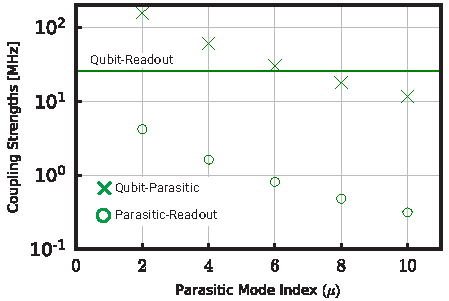
\includegraphics[width=\linewidth]{Supp_Fig/Coupling-strength.pdf}
    \caption{{\bf Absolute values of the coupling strengths.} $g_{\phi r}/2\pi$ (qubit-readout), $g_{\phi\mu}/2\pi$ (qubit-parasitic), $g_{\mu r}/2\pi$ (parasitic-readout), for various circuits. Coupling to odd parasitic modes is zero due to the symmetries of the circuit~\cite{viola2015collective}. The parasitic modes $\mu\in\{2,4,6\}$ couple to the qubit more strongly than the readout.}
    \label{fig:coupling-strength}
\end{figure}
\begin{enumerate}
    \item Total ground capacitance.
    \begin{enumerate}
        \item $H_1: E_t=(\frac{N-1}{E_g}+\frac{2}{E_{g1}}+\frac{2}{E_c})^{-1}=0.57 $ GHz
    \item $H_2: E_t=(\frac{N-1}{E_{g,j}}+\frac{2}{E_{g_p}}+\frac{1}{E_c})^{-1}$
    \item $H_3: E_t=(\frac{N-1}{E_{g,j}}+\frac{1}{E_{g_p}}+\frac{1}{E_c})^{-1}$
    \end{enumerate}
\item Qubit Charging energy ($4E_c^\phi \hat N_{\phi}^2$). 
    \begin{enumerate}
    \item $H_1:\bar{E}_c^\phi=(\frac{1}{4E_t}\Big(1-\frac{2}{3}\frac{(N+1)(N-1)}{N}\frac{E_t}{E_g}\Big)+\frac{1}{E_{C'}}+\frac{1}{NE_{C_j}})^{-1}=0.92 \ \mathrm{GHz}$.
    \item $H_2: \bar{E}_c^\phi=(\frac{1}{4E_t}\Big(1-\frac{E_t}{E_c}\Big)^2\Big[1-\frac{2}{3}\frac{N-1}{N}\Big]+\frac{1}{E_{C_p}}+\frac{1}{NE_{C_j}})^{-1}$. 
    \item  $H_3: \bar{E}_c^\phi=(\frac{1}{4E_t}\Big(1-\frac{E_t}{E_c}\Big)^2\Big[1-\frac{2}{3}\frac{N-2}{N-1}\Big]+\frac{1}{E_{C_p}}+\frac{1}{NE_{C_j}})^{-1}$.
    \end{enumerate}
    
\item Even Parasitic Mode Charging Energy  ($4E_{c,\mu}^e \hat N_{\mu}^2$). 
    \begin{enumerate}
    \item $H_1: \tilde{E}_{c,\mu}^{e}=(\frac{1}{E_{C_j}}+\frac{1}{4E_gs_\mu^2})^{-1}$ 
    \item $H_2:$ Same as $H_1$
    \item $H_3:$ Same as $H_1$
\end{enumerate}
     \item Qubit-Readout Coupling ($g_{\phi r}N_{\phi,\mathrm{ZPF}}N_{\mu,\mathrm{ZPF}}$).
    \begin{enumerate}
        \item $H_1: \frac{\tilde{E}_c^\phi}{E_c}$
        \item $H_2:\frac{\bar{E}_c^\phi}{E_c} \Big[\frac{(N+1)E_t}{2E_{g,j}}+\frac{E_t^2\tilde{E}_{c,\mu}^o}{8E_{g,j}^2E_c} \Big(\frac{c_\mu^2}{2Ns_\mu^4}\Big)\Big]$
        \item $H_3:\frac{\bar{E}_c^\phi}{E_c} \Big[\frac{NE_t}{2E_{g,j}}+\frac{E_t^2\tilde{E}_{c,\mu}^o}{8E_{g,j}^2E_c} \Big(\frac{c_\mu^2}{2(N-1)s_\mu^4}\Big)\Big]$
    \end{enumerate}
\item Qubit-Parasitic Coupling ($g_{\phi\mu}N_{\phi,\mathrm{ZPF}}N_{\mu,\mathrm{ZPF}}$)    
    \begin{enumerate}
        \item $H_1: \sqrt{\frac{2}{N}} \frac{\tilde{E}^\phi_c\tilde{E}^e_{c,\mu}c_\mu}{E_{g,j}s_\mu^2}$
        \item $H_2:\sqrt{\frac{2}{N}} \frac{\bar{E}^\phi_c\tilde{E}^{e}_{c,\mu}c_\mu}{E_{g,j}s_\mu^2}$
        \item $H_3:\sqrt{\frac{2}{N-1}} \frac{\bar{E}^\phi_c\tilde{E}^{e}_{c,\mu}c_\mu}{E_{g,j}s_\mu^2}$
    \end{enumerate}

\item Readout-Parasitic Coupling ($g_{\mu r}N_{\mu,\mathrm{ZPF}} V_{\mathrm{ZPF}}$)
    \begin{enumerate}
        \item $H_1: \frac{\tilde{E}^\phi_c\tilde{E}^e_{c,\mu}c_\mu}{4\sqrt{2N}E_{g,j}E_cs_\mu^2}$
        \item $H_2:\frac{\bar{E}^\phi_c\tilde{E}^{e}_{c,\mu}c_\mu }{4\sqrt{2N}E_{g,j}s_\mu^2E_c}\Big[\frac{(N+1)E_t}{2E_g} \Big]$
        \item $H_3:\frac{\bar{E}^\phi_c\tilde{E}^{e}_{c,\mu}c_\mu }{4\sqrt{2(N-1)}E_{g,j}s_\mu^2E_c}\Big[\frac{NE_t}{2E_{g,j}} \Big]$
    \end{enumerate}
   
\end{enumerate}

Zooming into Fig.~\ref{fig:circuit_choice}(c), we can see in Fig.~\ref{fig:coupling-strength} that for all three circuits the lowest three even modes $\mu=2,4,6$ couple to the qubit stronger than the readout. This observation is a backbone of our work; we find that because of this relatively large coupling strength, p-MIST rates may be significant in a broader fluxonium-based quantum computers.

In Fig.~\ref{fig:circuit_comp}, we show the dependence of charging energies and coupling constants on the number of junctions$N$ as well as the ground capacitance $C_g$. We find that the charging energies increase with decrease in $C_g$ and $N$. The parasitic charging energy is crucial in deciding the parasitic mode frequency $\omega_{\mu}$. A higher parasitic charging frequency relative to the readout frequency can lower the chances of p-MIST effects. Thus, we prefer large $C_g$ and $N$. The coupling strengths as shown in Fig.~\ref{fig:coupling-Floquet} induce all MIST effects. In particular, the parasitic-qubit coupling $g_{\phi\mu}$ is responsible for p-MIST effects. The parasitic-readout coupling $g_{\mu r}$ on the other hand only increases population  of the parasitic modes and is directly proportional to $g_{\phi\mu}$. We find that for low $g_{\phi\mu}$ a low $C_g$ and high $N$ is required. Thus, to reduce p-MIST effects the best strategy is to target for low parasitic ground capacitance in the JJA and high junction count.
\begin{figure}[t]
    \centering
    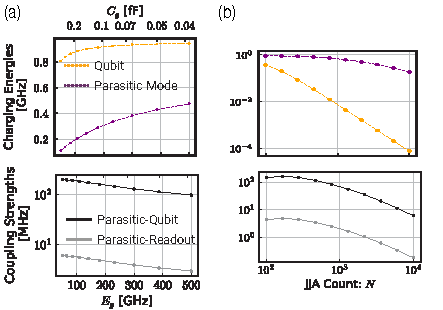
\includegraphics[width=\linewidth]{Supp_Fig/Circuit_comp.pdf}
    \caption{{\bf Dependence of coupling strengths and charging energies on circuit parameters.} (a) parasitic ground capacitance and (b) number of junctions in the array $N$. {\bf (Top row)} The qubit charging energy decides the frequency $\omega_{01}$ and the parasitic charging energy decides the parasitic mode frequency for mode $\mu=2$. {\bf (Bottom row)} give the plots for the coupling strengths of the parasitic mode to readout and qubit, respectively. All plots are obtained under linear JJA approximation.}
    \label{fig:circuit_comp}
\end{figure}

\paragraph{Variation in coupling strength.} Note that, changing $N$ changes the target inductance of the qubit. When increasing $N$, we need to proportionally increase the energies $E_{J_j}$ to fix the inductive energy of the qubit ($E_L=E_{J_j}/N$). However, $E_{J_j}$ is constrained within a typical fabrication process window, capping the maximum $E_{L}$. This further supports the large $N$ approximation $\tilde{E}_{c,\mu}^e\approx 4E_{g,j}s_\mu^2$ (see Eq.~\ref{eq:parasitic}). Thus, the number of junctions $N$ can be optimized to decrease $g_{\phi\mu}$ while keeping $E_L$ constant. 

However, increasing $N$ while keeping $E_L, E_{g,j}$ constant also decreases the parasitic charging energy (see Fig.~\ref{fig:circuit_comp} in App.~\ref{app:coupling}). For large $N$ and small $\mu$ limit,
\begin{align}
\tilde{E}_{c,\mu}^e\propto 1/N^2,  \label{eq:dep2} 
\end{align}
which corresponds to lowering the parasitic mode frequency $\omega_\mu$ with increasing $N$. This outcome is generally not favorable towards reducing p-MIST, as discussed in the next section. However, in the absence of any coupling to the qubit $g_{\phi\mu}$, even a low frequency parasitic mode will be of no consequence to p-MIST effects.

\paragraph{Variation in parasitic charging energy.}  Eqs.~\ref{eq:dep1}-\ref{eq:dep2} show that, for large $N$ and small $\mu$ limit, $\omega_\mu^e$ is inversely proportional to $N^2$ and $C_{g,j} \ \mathrm{[fF]}=\frac{19.4}{E_{g,j} \ \mathrm{[GHz]}}$ (see Fig.~\ref{fig:circuit_comp} in App.~\ref{app:coupling}). Thus, again, a smaller parasitic ground capacitance $C_{g,j}$ increases the parasitic mode charging energy, thus increasing its frequency, favorably. However, in contrast with the case of coupling strength $g_{\phi\mu}$, a larger $N$ leads to lower frequencies for these modes, which is unfavorable since it decreases the gap between the between $\omega_d$ and $\omega_\mu$. We already discussed the complications of changing the ground capacitance $C_{g,j}$ in the previous discussion of coupling strengths above. The impact of decreasing $N$ would require careful consideration of increased nonlinearity of the parasitic modes as well as increased coupling strengths.


\subsection{Fluxonium Qubit Hamiltonian}
\sh{check for units to be $\hbar=1$}
We now discuss the Fluxonium qubit Hamiltonian, through a detailed consideration of its charge matrix elements and the dispersive shifts on the qubit induced by the parasitic modes and readout. This dispersive Hamiltonian is derived using the Schrieffer-Wolff approximation~\cite{viola2015collective}. The qubit Hamiltonian $H_{\phi}$ (see Eq.~\ref{eq:Hphi}) is diagonalized in the Fock state basis, where we have used the standard bosonic operators
 \begin{equation} \hat x=x_{\mathrm{ZPF}}(a+a^\dagger)=\hat N_{\phi}/ N_{\phi,\mathrm{ZPF}}
 \end{equation}
 and 
 \begin{equation} \hat p=-ip_{\mathrm{ZPF}}(a-a^\dagger)=\hat \phi/\phi_{\mathrm{ZPF}}.
 \end{equation}
such that $[\hat x,\hat p]=i$.
\paragraph{Charge Matrix Elements for $H_1,H_2,H_3$:}
Here, using the approximations described in App.~\ref{app:alt_circuits}, we calculate the charge matrix elements for the qubit mode. We observe that with increasing final state ($f$), the charge matrix elements with respect to the ground and first two excited states follow a decreasing trend, approximately exponential. This exponential decrease to $10^{-10}$ motivates our truncation of the fluxonium potential up to $30$ levels for the Floquet simulations of Sec.~\ref{sec:MIST}.
\begin{figure}[hbt]
    \centering
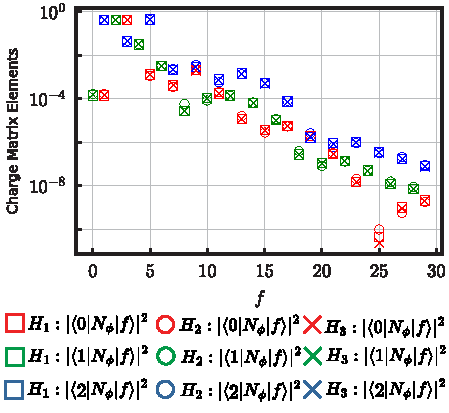
\includegraphics[width=0.45\textwidth]{Supp_Fig/Charge_Matrix.pdf}
    \caption{{\bf Charge matrix 
 elements (squared) for all three circuits.} Note that we use $\langle f|N_\phi|f'\rangle=iN_{\phi,\mathrm{ZPF}}\langle f|(a-a^\dagger)|f'\rangle$ where $N_{\phi,\mathrm{ZPF}}=\frac{1}{\sqrt{2}}\Big(E_{J,j}/8NE_C\Big)^{1/4}$. The charge matrix elements between parity conserving states is zero (points not seen in log plot) due to the symmetry of cosine potential at $\varphi_\mathrm{ext}=0.5\Phi_0$, where $\Phi_0$ is the flux quantum.}
    \label{charge-matrix}
\end{figure}


\paragraph{Dispersive Hamiltonian}\label{app:dispersive}
Next, we extract the qubit parameters quoted in Table~\ref{tab:readout_params}, for example, the dispersive shift of the qubit due to the parasitic modes $\chi_{\phi\mu}$ and the readout mode $\chi_{\phi r}$~\cite{viola2015collective}. These variables were used to generate Fig.~\ref{fig:dephasing} in the main text. For this purpose, we first give the qubit Hamiltonian in the dispersive regime~\cite{viola2015collective},

\allowdisplaybreaks{
\begin{align}
    H/\hbar&=\frac{\omega_q}{2}\sigma_z+\sum_{\mu}(\omega_\mu+k_\mu) a_\mu^\dagger a_\mu
    +\omega_r a_r^\dagger a_r\nonumber\\ &\quad +\chi_{r,\phi}\sigma_z a_r^\dagger a_r
    +\sum_{\mu}\chi_{\mu,\phi}\sigma_z a_\mu^\dagger a_\mu
   \nonumber\\&\quad +\sum_{\mu}\chi_{r\mu} a_\mu^\dagger a_\mu a_r^\dagger a_r\\
   &=\frac{\omega_q}{2}\sigma_z+\Big(\omega_r +\chi_{r\phi}\sigma_z\Big)a_r^\dagger a_r\nonumber\\&+\sum_{\mu}\Big(\omega_\mu+k_\mu+\chi_{r\mu}a_r^\dagger a_r+\chi_{\mu\phi}\sigma_z\Big) a_\mu^\dagger a_\mu\label{eq:dispersive}
\end{align}
where the lamb shift is given by,
\begin{align}
   k_{\mu\in 2\mathbb{Z}}&=16E_{C_r}^2\sqrt{\frac{E_{L_r}}{32E_{C_r}}}\sqrt{\frac{E_{J_j}}{32E_C^e}}\Bigg[\frac{g_{r\mu}^2}{\omega_\mu-\omega_r}\Bigg]
\end{align}
$\le\mathcal{O}(10^{-8})$. 
In Eq.~\ref{eq:dispersive} the qubit frequency is given by $\omega_{01}=\epsilon_1-\epsilon_0$
\begin{align}
    &=-|\langle 0|p_\phi|1\rangle|^2\Bigg[16g_{r\phi}^2E_{C_r}^2\sqrt{\frac{E_{L_r}}{32E_{C_r}}}\frac{2\epsilon_{01}}{\epsilon_{01}^2-\omega_r^2}\nonumber\\ &\quad+\sum_\mu\Bigg\{g_{\mu\phi}^2\sqrt{\frac{E_{J_j}}{32\tilde{E}_{C,\mu}^e}}\frac{2\epsilon_{01}}{\epsilon_{01}^2-\omega_\mu^2}\Bigg\}\Bigg]\nonumber\\&-\sum_{l>1}16g_{r\phi}^2E_{C_r}^2\sqrt{\frac{E_{L_r}}{32E_{C_r}}}\Bigg[\frac{|\langle 0|p_\phi|l\rangle|^2}{\epsilon_{0l}-\omega_r}\nonumber\\&-\frac{|\langle 1|p_\phi|l\rangle|^2}{\epsilon_{1l}-\omega_r}\Bigg]+\sum_{l>1,\mu}\Bigg\{g_{\mu\phi}^2\sqrt{\frac{E_{J_j}}{32\tilde{E}_{C,\mu}^e}}\times\nonumber \\&\quad\Bigg[\frac{|\langle 0|p_\phi|l\rangle|^2}{\epsilon_{0l}-\omega_\mu}-\frac{|\langle 1|p_\phi|l\rangle|^2}{\epsilon_{1l}-\omega_\mu}\Bigg]\Bigg\}
\end{align}
Here the second summand over $\mu$ is the correction $\delta_{\omega_{01}}$ to the qubit frequency due to parasitic modes. For the parameters used in Table~\ref{tab:circuit_params}, which yields $\omega_{01}/2\pi=30 \ \mathrm{MHz}$ the frequency corrections for circuits $H_1,H_2,H_3$ are $\delta\omega_{01}/2\pi=0.4 \ \mathrm{MHz},0.45 \ \mathrm{MHz},0.41 \ \mathrm{MHz}$, respectively. 

The dispersive shift due to the readout mode is given by,
\begin{align}
\chi_{\phi r}&=16g_{r\phi}^2E_{C_r}^2\sqrt{\frac{E_{L_r}}{32E_{C_r}}}\frac{2\epsilon_{01}}{\epsilon_{01}^2-\omega_r^2}|\langle 0|p_\phi|1 \rangle|^2\nonumber\\
   &+16g_{r\phi}^2E_{C_r}^2\sqrt{\frac{E_{L_r}}{32E_{C_r}}}\Bigg[\sum_l|\langle 0|p_\phi|l \rangle|^2\frac{\epsilon_{0l}}{\epsilon_{0l}^2-\omega_r^2}\nonumber\\&\quad-\sum_l|\langle 1|p_\phi|l \rangle|^2\frac{\epsilon_{1l}}{\epsilon_{1l}^2-\omega_r^2}\Bigg]
\end{align}
and the dispersive shift due to the parasitic mode is given by,
\begin{align}  
   \chi_{\phi\mu}&=g_{\mu\phi}^2\sqrt{\frac{E_{J_j}}{32\tilde{E}_{C,\mu}^e}}\frac{2\epsilon_{01}}{\epsilon_{01}^2-\omega_\mu^2}|\langle 0|p_\phi|1 \rangle|^2\nonumber\\
   &+g_{\mu\phi}^2\sqrt{\frac{E_{J_j}}{32\tilde{E}_{C,\mu}^e}}\Bigg[\sum_l|\langle 0|p_\phi|l \rangle|^2\frac{\epsilon_{0l}}{\epsilon_{0l}^2-\omega_\mu^2}\nonumber\\&\quad-\sum_l|\langle 1|p_\phi|l \rangle|^2\frac{\epsilon_{1l}}{\epsilon_{1l}^2-\omega_\mu^2}\Bigg]
\end{align}
}
For the parameters in Table~\ref{tab:circuit_params},  we plot $\chi_{\phi\mu},\chi_{\phi r}$ for all three circuits in Fig.~\ref{fig:dispersive-shift}. 
\begin{figure}[htb]
    \centering
    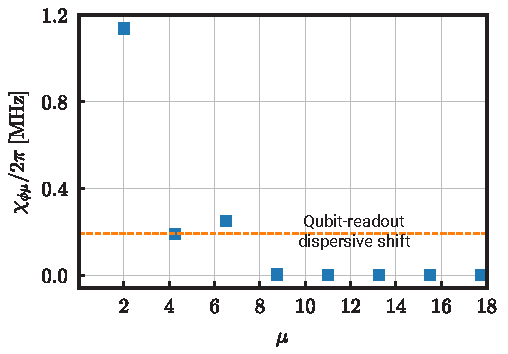
\includegraphics[width=0.45\textwidth]{Supp_Fig/dispersive_shift.pdf}
    \caption{ {\bf The dispersive shift induced on the qubit due to the parasitic mode $\mu$.} The three grounding configurations, parallel circuit ($H_1$), floating Fluxonium ($H_2$), and grounded fluxonium ($H_3$) shown in Figs.~\ref{fig:circuit_comp}(a-c) yield the same values. Dashed lines in the same color code represent the dispersive shift ($\sim $) induced by the readout resonator on the qubit.}
    \label{fig:dispersive-shift}
\end{figure}

\section{Driven Fluxonium Circuit}\label{app:MIST}
Here, we discuss the several analysis techniques to study MIST effects used in this work. We begin with the derivation of $H_{s.c.}$ in Eq.~\ref{eq:drive}. Then we discuss and justify the Hilbert space truncation, as well as approximations used for Floquet simulations in Sec.~\ref{sec:MIST}.
\subsection{Semi-classical Approximation}\label{app:semi-classical}
\sh{include the derivation}
\subsection{Approximations for Numerical Modeling}\label{app:numerics}
We use the following three approximations in our work.
\begin{itemize}
    \item \textbf{Restriction to $\mu=2$}. We restrict our analyses to only include the lowest-frequency, even parasitic mode. This mode couples most strongly to the qubit and the readout as evident from Fig.~\ref{fig:coupling-strength}(d). This assumption reduces the Hilbert space size for feasible study. 

    \item \textbf{Semi-classical drive approximation.}  We treat the readout resonator classically as described in Refs.~\cite{xiao2023diagrammatic,dumas2024unified,cohen2023reminiscence,khezri2023measurement}, eliminating the readout mode states from our numerical simulation. This approximation is again necessary to restrict the Hilbert space size to values feasible for numeric study.
    
    \item \textbf{Linear JJA Approximation.} We assume that the parasitic modes are linear, due to the large $E_{J_j}/E_{C_j} \sim 200$ ratio. Nonlinear corrections to our results is beyond the scope of this work. For details on how nonlinear corrections affect different circuit energies, we direct the readers to Ref.~\cite{viola2015collective}. 
    \item \textbf{Truncation.} We note that the charge matrix elements connecting the fluxonium qubit ground states to excited states decreases roughly exponentially with increasing excited state number. With this observation, shown in Fig.~\ref{charge-matrix}, as well as our assumptions above, we truncate the Hilbert space dimensions to $30\otimes 10$. That is, we assume $30$ levels in the fluxonium qubit mode and $10$ levels in the parasitic mode. 
    \end{itemize}
    Note that for the conclusions drawn in this paper, we are only interested in identifying the existence of p-MIST processes, and do not claim to quantify how many such transitions can be present. Hence, with this truncation we only examine the excitations to $0-2$ levels in the parasitic mode and $0-20$ in the fluxonium subspace in Figs.~\ref{fig:Floquet},~\ref{fig:Flo_low},~\ref{fig:coupling-Floquet}. In this appendix we will show the results for truncating the Hilbert space to $20
    times 5$ levels in the two modes and $30
    times 10$, showing the convergence of the MIST results.

\sh{Include the 30 X 10 as well as 20 X 3}

\subsection{Floquet Simulations}
\paragraph{Stark shift:}\label{app:stark-shift}
To observe a state transition the primary requirements are high charge matrix elements and low energy difference. The eigen-energies of the states in question are changed with an increase in the number of readout photons or, in this case, the drive strength. In this section, we compute the Stark shifted eigen-energies which facilitates the prediction of an avoided crossing using a first-order perturbative approach, given $\bar n_r, \omega_r$ and the charge matrix elements.  Let $\ket{i}$ be a state in the eigenspace of $H_{int}=H_\phi+H_{\mu=2}+g_{\phi\mu}\hat N_\phi\hat N_\mu$. Following derivations in App.~\ref{app:Hamiltonian}, the Stark-shift in the energy of state $\ket{i}$ at an average number of readout photons $\bar n_r$ is given by
\begin{align}
    \chi_i(\bar n_r)=2\bar n_r\sum_{f}\omega_{if}\Big[\frac{g_{\phi r}|\braket{i|\hat N_\phi|f}|^2}{\omega_d^2-\omega_{if}^2}+\frac{g_{\mu r}|\braket{i|\hat N_\mu|f}|^2}{\omega_d^2-\omega_{if}^2}\Big]\label{eq:stark}
\end{align}
 Here $\omega_{if}=E_f-E_i$ denote the energy difference in the eigen-energies of the state $\ket{i}$. The impact due to the second term is much smaller than the first term, and hence $g_{\phi r}$ primarily governs this Stark shift.
 \begin{figure}
     \centering
     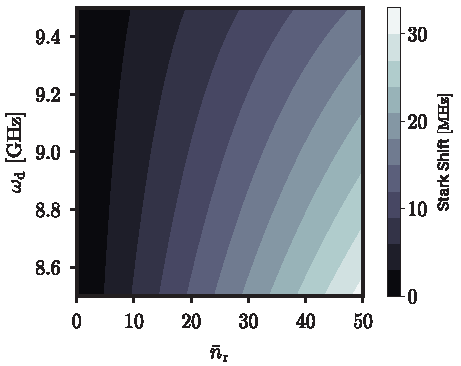
\includegraphics[width=\linewidth]{Supp_Fig/Stark-shift.pdf}
     \caption{Stark shift in different energy levels for readout computed using Eq.~\ref{eq:stark} for energy level $\ket{\tilde{0},\tilde{0}}$. We have verified that Stark shift on the excited energy levels $\ket{\tilde{1},\tilde{0}}$ and $\ket{\tilde{2},\tilde{0}}$ are also upper bounded by $50$ MHz for the ranges considered in x- and y-axes in this plot.}
     \label{fig:stark-shift}
 \end{figure}

\paragraph{Population exchange and quasienergies:}\label{app:Floquet-trans}
Below we plot the population exchange and quasienergy probabilities for all transitions captured in Fig.~\ref{fig:Floquet} and Table~\ref{tab:p-MIST} for states $\ket{\tilde{0},\tilde{0}}$ (see Fig.~\ref{fig:Trans0}), $\ket{\tilde{1},\tilde{0}}$ (see Fig.~\ref{fig:Trans1}) and $\ket{\tilde{2},\tilde{0}}$ (see Fig.~\ref{fig:Trans2}). We will comment on some special types of transitions explicitly here.

\begin{itemize}
    \item Transition $(2)$ has two crossings, one that takes place at $\bar n_r=14$ and another at $\bar n_r=48$. The states $\ket{\tilde{4},\tilde{2}}$ and $\ket{\tilde{14},\tilde{2}}$ hybridize first and then the resulting state hybridizes with the computational state $\ket{\tilde{0},\tilde{0}}$.
    \item Transitions $(3,4)$ show a branch bunching scenario, as quoted in Ref.~\cite{dumas2024unified} for the case of positive detuning. However, in this case we note that both branch bunching and crossings were observed in the negative detuning case. Such branch bunching occurs when the drive frequency $(\omega_d)$ is equal to the transition frequency of two states $i,j (\omega_{ij})$. In the presence of parasitic mode, there are multiple states ($\ket{\tilde{i},\tilde{\mu
    }}$ and $\ket{\tilde{j},\tilde{\mu}}$ for various $\mu$) such that $\omega_d=\omega_{ij}$ is the resonant frequency for the observation of bunching between the two states.
    \item In transitions $(9,11,12)$ the states do not return to the same population as the initial states. This is the case because we are plotting the bare fluxonium and parasitic mode operators $\braket{\bar n_\phi},\braket{\bar n_\mu}$. We make this choice to show the impact of p-MIST effects on the bare fluxonium population since the parasitic modes have been ignored in most previous fluxonium analyses.
    \item Finally, in transition $(14)$ we again see two crossings. In the absence of qubit-parasitic coupling $g_{\phi\mu}$ this transition is only carried out between  $\ket{\tilde{17},\tilde{0}}$ and $\ket{\tilde{2},\tilde{0}}$. However, in the presence of parasitic modes $\ket{\tilde{17},\tilde{0}}$ hybridizes with $\ket{\tilde{5},\tilde{1}}$ which then has a branch crossing with $\ket{\tilde{2},\tilde{0}}$. Thus, in this case we see that ignoring parasitic modes can lead to wrong state predictions which could affect the qubit reset post measurement.
\end{itemize}

\paragraph{Landau-Zener probabilities:}\label{app:LZ}
We compute the Landau-Zener probabilities in Sec.~\ref{sec:LZ} numerically using the quasienergies from the Floquet simulations, and analytically, using the Stark-shifted eigen-energies. In this case, we use a time-dependent readout photon number, where $\bar n_r$ varies as $\bar n_r=50(1-e^{-\kappa t/2})^2$, to emulate change in readout photons from dissipation~\cite{dumas2024unifie,khezri2023measurement}. The numerical calculations use the probability for Landau-Zener transitions given in~\cite{ikeda2022floquet}, for an avoided crossing observed between states $\ket{i},\ket{f}$ of
\begin{align}
    P_{LZ}&=\exp{\Big[-\frac{\pi \Delta_{ac}^2}{2v}\Big]},\\
    \text{where } v&=\sqrt{2\Delta_{ac}\Big|\frac{d^2\epsilon_f}{d\sqrt{\bar{n}_r(t)}^2}\Big|_{t_{ac}}}\frac{d\sqrt{\bar{n}_r(t)}}{dt}|_{t_{ac}}\Big .
\end{align}
Here, the variable $\epsilon_j$ is the numerically-computed quasi-energy obtained from Floquet simulations, while $\Delta_{ac}$ refers to their quasi-energy difference at avoided crossing. 

\section{Alternative Circuit}\label{app:alt_circuit1}
Here, we give the circuit parameters (Table~\ref{tab:circuit_params_Will}), coupling strengths (Fig.~\ref{fig:coupling-strength-Will}), charge matrix elements (Fig.~\ref{fig:charge-matrix-Will}) and state transition quasienergies shown in Figs.~\ref{fig:Floquet1} and Fig.~\ref{fig:011_Will}. 
%The truncation for these simulations uses the same justification and assumptions as App.~\ref{app:numerics}. 
\begin{table}[htb]
\centering
\begin{tabular}{|c|c|c|c|c|c|c|c|c|c|}
    \hline
     $N$ & $\varphi_{ext}$ & $E_{J_p}$ & $E_{C_p}$ & $E_C$ & $E_{C_j}$ & $E_{J_j}$ & $E_{C_{g,j}}$ & $E_{C_{g,p}}$ & $E_c$ \\
    \hline
    $102$ & $0.5\Phi_0$ & $6.20$ & $1.24$ & $4.28$ & $0.74$ & $81.6$ & $194$ & $1.94$ & $19.40$ \\
    \hline
\end{tabular}
\caption{Circuit parameters for Fig.~\ref{fig:Floquet1}(a) inspired by Ref.~\cite{ding_high-fidelity_2023}. All energies are given in GHz. Here $\Phi_0=h/2e$ denotes the magnetic flux quantum. The capacitive energies $E_{C'}=\frac{19.4}{{C'}(fF)} \ \mathrm{GHz}$ are computed from the corresponding capacitances $C'$.}
\label{tab:circuit_params_Will}
\end{table}

The coupling strengths in this circuit are similar to those evaluated for our original circuit parameters, in Fig.~\ref{fig:coupling-strength}.
\begin{figure}[htb]
    \centering
    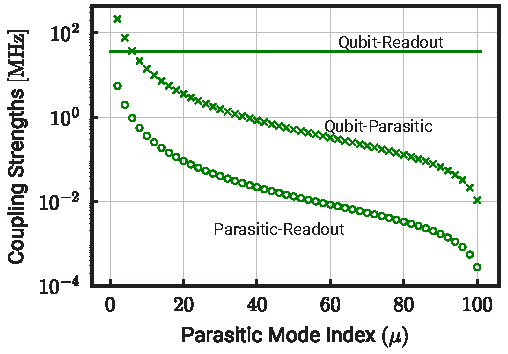
\includegraphics[width=\linewidth]{Supp_Fig/Coupling-Will.pdf}
    \caption{{\bf Absolute values of the coupling strengths.} $g_{\phi r}/2\pi$ (qubit-readout), $g_{\phi\mu}/2\pi$ (qubit-parasitic), $g_{\mu r}/2\pi$ (parasitic-readout), for various circuits. Coupling to odd parasitic modes is zero due to the symmetries of the circuit~\cite{viola2015collective}. The parasitic modes $\mu\in\{2,4,6\}$ couple to the qubit more or as strongly as the readout.}
    \label{fig:coupling-strength-Will}
\end{figure}

We find in Fig.~\ref{fig:charge-matrix-Will} that the charge matrix elements of the second circuit analyzed in Sec.~\ref{Will_circuit} has a faster decrease with increasing excited state levels. This could be indicative of the fact that such a circuit will see lower MIST effects as observed in Fig.~\ref{fig:Floquet1}(c). 
\begin{figure}[htb]
    \centering
    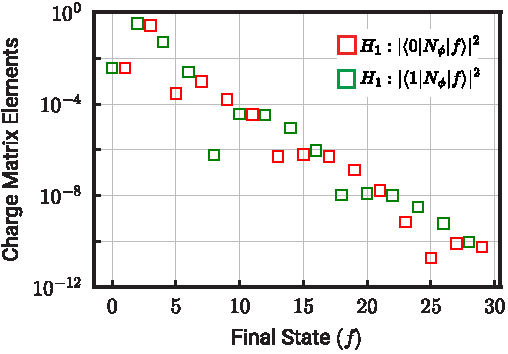
\includegraphics[width=\linewidth]{Supp_Fig/Charge-matrix-Will.pdf}
    \caption{{\bf Charge Matrix 
 Elements (squared) for all three circuits.} Note that in the equations below we substitute $\langle i|N_\phi|f\rangle=iN_{\phi,\mathrm{ZPF}}\langle i|(a-a^\dagger)|f\rangle$ where $N_{\phi,\mathrm{ZPF}}=\frac{1}{\sqrt{2}}\Big(E_{J,j}/8NE_C\Big)^{1/4}$. The charge matrix elements between odd-odd or even-even is zero (points not seen in log plot) due to the symmetry of cosine potential at $\varphi_\mathrm{ext}=0.5\Phi_0$, where $\Phi_0$ is the flux quantum. Here $H_1$ denotes the parallel circuit in Fig.~\ref{fig:circuit_choice}(a).}
    \label{fig:charge-matrix-Will}
\end{figure}

Finally, we plot the p-MIST effect observed in the Floquet simulations for this alternative circuit in Fig.~\ref{fig:011_Will}. We perform a branch analysis of the initial state $\ket{\tilde{0}, \tilde{0}}$ and observe a transition to $\ket{\tilde{4},\tilde{1}}$, as described in the main text. 

 \begin{figure}[htb]
    \centering
    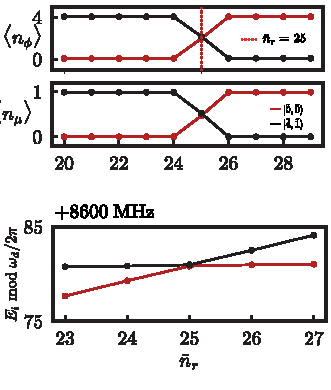
\includegraphics[width=\linewidth]{Supp_Fig/Floquet_Will_landscape.pdf}
    \caption{{\bf Examples of p-MIST using transitions for the alternative circuit in Fig.~\ref{fig:Floquet1}(c) of Sec.~\ref{Will_circuit}.} involving the states $\ket{\tilde{0},\tilde{0}}\leftrightarrow\ket{\tilde{4},\tilde{1}}$, with maximum overlap to the un-hybridized state $\ket{k}_\phi\otimes\ket{n}_{\mu=2}$. \textbf{Top row:} Qubit mode average occupation $\braket{n_\phi}$. \textbf{Middle row:} Parasitic mode average occupation $\braket{n_\mu}$. \textbf{Bottom row:} Quasi-energies (solid) from Floquet simulations showing avoided crossings. Plots are extracted from numerical data used in Fig.~\ref{fig:Floquet}. The data points are connected by lines for visual aid.}
    \label{fig:011_Will}
\end{figure}

%Finally, we focus on the rate of this p-MIST process using Landau Zener calculations as follows in Fig.??.
%\sh{Add Landau Zener plot}
\begin{figure*}
    \centering
    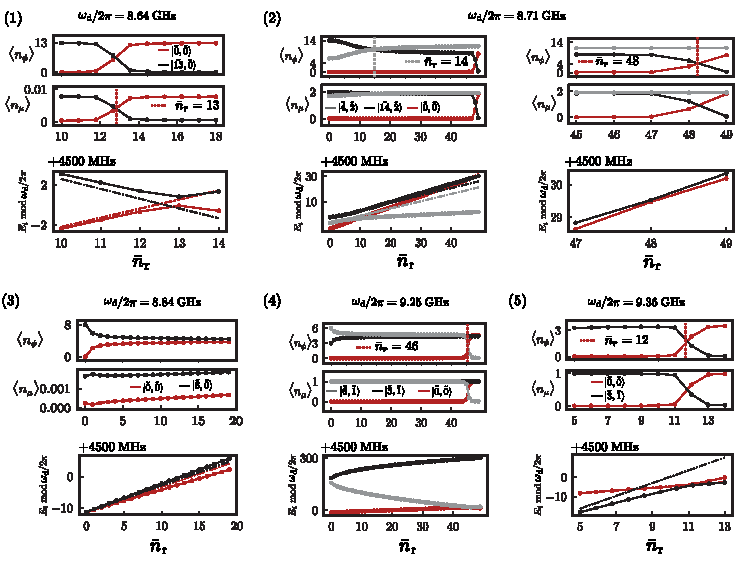
\includegraphics[width=1.0\textwidth]{Supp_Fig/Trans0.pdf}
    \caption{MIST processes from Table~\ref{tab:p-MIST} involving the $\ket{\tilde{0},\tilde{0}}$ state in rows indexed by figure numbering. (Top row) Fluxonium subspace $\braket{n_\phi}$. (Middle) Parasitic mode subspace $\braket{n_\mu}$ (Bottom) Stark-shifted eigen-energies (dashed) and quasi-energies (solid) from Floquet simulations, corresponding to the initial state $i$ as per the legend. Inset shows avoided crossing of quasi-energies. Floquet results are extracted from numerical data used for Fig.~\ref{fig:Floquet}. Note that MIST in figure $(2)$ is split into two figures in order to capture the two consecutive transitions involved.}
    \label{fig:Trans0}
\end{figure*}
\begin{figure*}
    \centering
    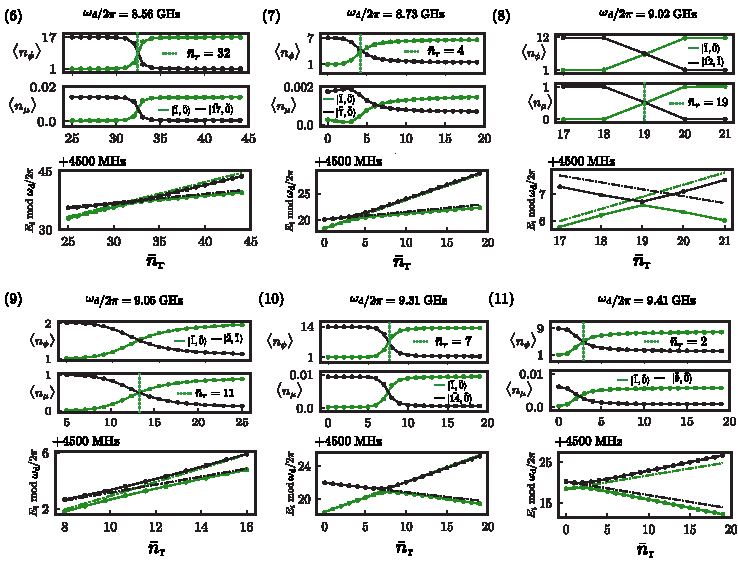
\includegraphics[width=1.0\textwidth]{Supp_Fig/Trans1.pdf}
    \caption{MIST processes from Table~\ref{tab:p-MIST} involving the $\ket{\tilde{1},\tilde{0}}$ state in rows indexed by figure numbering. (Top row) Fluxonium subspace $\braket{n_\phi}$. (Middle) Parasitic mode subspace $\braket{n_\mu}$ (Bottom) Stark-shifted eigen-energies (dashed) and quasi-energies (solid) from Floquet simulations, corresponding to the initial state $i$ as per the legend. Inset shows avoided crossing of quasi-energies. Floquet results are extracted from numerical data used for Fig.~\ref{fig:Floquet}.}
    \label{fig:Trans1}
\end{figure*}
\begin{figure*}
    \centering
    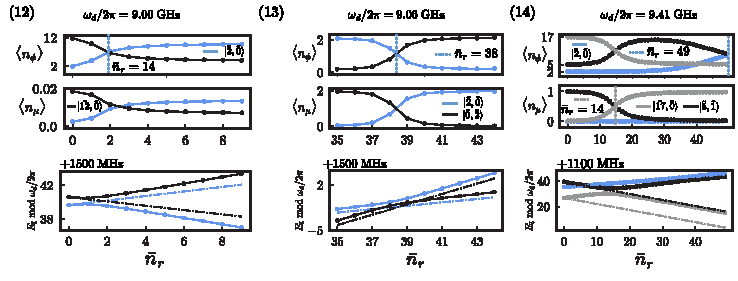
\includegraphics[width=1.0\textwidth]{Supp_Fig/Trans2.pdf}
    \caption{MIST processes from Table~\ref{tab:p-MIST} involving the $\ket{\tilde{2},\tilde{0}}$ state in rows indexed by figure numbering. (Top row) Fluxonium subspace $\braket{n_\phi}$. (Middle) Parasitic mode subspace $\braket{n_\mu}$ (Bottom) Stark-shifted eigen-energies (dashed) and quasi-energies (solid) from Floquet simulations, corresponding to the initial state $i$ as per the legend. Inset shows avoided crossing of quasi-energies. Floquet results are extracted from numerical data used for Fig.~\ref{fig:Floquet}.}
    \label{fig:Trans2}
\end{figure*}

\clearpage
\begin{itemize}
    \item Units of g is an outstanding issue: momentum or charge coefficient?
    \item p-MIST or PIST
    \item some sub-figures have subheadings some do not
    \item shorter conclusion
\end{itemize}
\clearpage
\bibliography{refs.bib} 
\end{document}

